%\documentstyle[12pt,accents]{article}

\documentclass[11pt]{article}

\usepackage{graphicx}
\usepackage{epsfig}
\usepackage{amssymb}
\usepackage{amsmath}
\usepackage{amsthm}
\usepackage{amscd}
%\usepackage[latin1]{inputenc}
%\usepackage{minitoc}

\usepackage[english]{babel}
\usepackage[utf8]{inputenc}
%\usepackage[usenames]{color}
%\usepackage{color}
\usepackage[usenames,dvipsnames,svgnames,table]{xcolor}
\usepackage{latexsym}
\usepackage{graphicx}
\usepackage{geometry}
\usepackage{accents}
\usepackage{url}

\usepackage[framemethod=tikz]{mdframed}
\usepackage{tikzpagenodes}
\usetikzlibrary{calc}

%http://tex.stackexchange.com/questions/107191/indented-box-that-split-in-multiple-pages
\mdfdefinestyle{mysquare}{%
  leftmargin=0pt,
  rightmargin={\dimexpr4pt+2ex\relax},
  innertopmargin=2\baselineskip,
  skipabove={\dimexpr0.5\baselineskip+\topskip\relax},
  skipbelow={\dimexpr0.5\baselineskip+\topskip\relax},
  singleextra={% Single extra applies when it fits in a single page
  \path let \p1=(P), \p2=(O)
    in node[font=\bfseries] at ([yshift=-2ex]0.5*\x1-\x2,\y1) {Solution};
  \fill[black] ([xshift=2pt,yshift=2pt]P) rectangle ++(1ex,1ex);
  \fill[black] ([xshift=-2pt,yshift=-2pt]O) rectangle ++(-1ex,-1ex);
  \fill[black] ([xshift=-2pt,yshift=2pt]O|-P) rectangle ++(-1ex,1ex);
  \fill[black] ([xshift=2pt,yshift=-2pt]O-|P) rectangle ++(1ex,-1ex);
  },
  firstextra={% First extra applies on the first page when it doesn't fit in one page
  \path let \p1=(P), \p2=(O)
    in node[font=\bfseries] at ([yshift=-2ex]0.5*\x1-\x2,\y1) {Solution};
  \fill[fill=black] ([xshift=2pt,yshift=2pt]P) rectangle ++(1ex,1ex);
  \fill[black] ([xshift=-2pt,yshift=2pt]O|-P) rectangle ++(-1ex,1ex);
  },
  secondextra={% First extra applies on the last page when it doesn't fit in one page
  \fill[fill=black] ([xshift=2pt,yshift=-2pt]O-|P) rectangle ++(1ex,-1ex);
  \fill[black] ([xshift=-2pt,yshift=-2pt]O) rectangle ++(-1ex,-1ex);
  }
}
\newmdenv[style=mysquare]{solution}

\newcommand{\maxi}{\mbox{maximiser}}
\newcommand{\mini}{\mbox{minimiser}}
\newcommand{\xopt}{\ensuremath{x^*}}
\DeclareMathOperator{\newdiff}{d} % use \dif instead
\newcommand{\dif}{\newdiff\!}

\newcommand{\nosolution}
{Cet exercice ne contient pas encore de solution.
Vous êtes invité à nous en soumettre une à l'adresse suivante
\begin{center}
\url{https://github.com/blegat/LINMA1702-exercices}
\end{center}
ou par mail.}

\parindent0mm

\setlength{\textwidth}{15cm}
\setlength{\oddsidemargin}{0.50cm}
\setlength{\textheight}{8.7in}
\setlength{\topmargin}{-0.5in}

\newcommand{\R}{{\mbox{\bf R}}}

\newcommand{\head}{{\parindent 0pt  V. Blondel \hfill INMA1702 \\}}

% Pour les graphes des espaces admissibles
% http://tex.stackexchange.com/questions/6364/how-to-plot-polygon-using-tikz
\usepackage{tikz}
\usepackage{mathtools}
\def\nudge{.5}
%\tikzset{axis/.style={ultra thick, Red!75!black, -latex, shorten <=-\nudge cm, shorten >=-2*\nudge cm}}
\tikzset{axis/.style={thick, Red!75!black, -latex, shorten <=-0.5*\nudge cm, shorten >=-\nudge cm}}
\tikzset{line/.style={thick,Green}}
\tikzset{hash/.style={pattern=north west lines, pattern color=blue}}
\usetikzlibrary{patterns}

\author{Vincent Blondel\\
Université catholique de Louvain}

\title{INMA1702. Mod\`eles et m\'ethodes d'optimisation
  \\
Exercices (partie optimisation linéaire)}

\begin{document}

\date{Année 2007-2008}

\maketitle

\begin{center}
\textbf{Code source et bug tracker}\\
\url{https://github.com/blegat/LINMA1702-exercices}
\end{center}

\newpage

%******************************************************************************

\tableofcontents

\newpage

%******************************************************************************

\section{Problèmes d'optimisation linéaire}

Soit le problème

$$
\begin{array}{ll}
  \mini   &  f(x_1, \ldots, x_n) \\
  \mbox{sous la contrainte} &  (x_1, \ldots, x_n)  \in \Omega
\end{array}
$$


Les scalaires $x_1, \ldots, x_n \in \R$ sont les \emph{variables de décision}, $f$  est la \emph{fonction objectif}
(on parle volontier de \emph{fonction coût} pour un problème de minimisation et de \emph{fonction profit} pour un problème de maximisation), et
$\Omega$ est le \emph{domaine admissible}. Un élément de $\R^n$ est une \emph{solution}, c'est une \emph{solution admissible}   si
$x
\in \Omega$. Si la solution admissible
$x^\star$ est telle que
$f(x^\star) \leq f(x)$ pour toute autre solution admissible
$x$,  la solution $x^\star$ est \emph{optimale}. L'\emph{objectif optimal}   est alors donné par
$f(x^\star)$. Lorsqu'il existe, le coût optimal est unique. Par contre, il peut y avoir de nombreuses solutions optimales et l'ensemble des solutions
optimales peut être non borné. Si pour tout
$K$ il existe une solution admissible $x \in \Omega$ telle que $f(x) \leq K$, le coût est dit \emph{non borné}. On
dit aussi que le  coût est \emph{égal à
$-\infty$}.\\

\newpage



\begin{enumerate}


  \item Un étudiant dispose de 100 heures de travail pour étudier les examens A, B et C. Il pense gagner par heure de travail et par
    cours: 1/5 de points pour le cours A, 2/5 de points pour le cours B et 3/5 pour le cours C. Chaque examen est coté sur 20. Les
    exercices de ces cours comptent pour la moitié de la cote finale. Ses résultats pour les exercices lui ont été communiqués. Il a
    obtenu 12/20 pour A, 12.5/20 pour B et 13.4/20 pour C.  L'étudiant doit obtenir au minimum une cote globale de 10/20 pour chaque cours. Tous
    les cours ont la même pondération et l'étudiant désire obtenir la  moyenne la plus élevée possible.  Formulez ce problème comme un problème d'optimisation
    linéaire (solution lors d'une séance ultérieure).
    \begin{solution}
      Soient $x_{A}, x_{B}~et~x_{C}$ le nombre d'heures consacrées aux cours $A, B$ et $C$. La valeur de la fonction est sur $20$.\\
      $$6,317 - min -\frac{1}{3}(\frac{x_{A}}{5} + \frac{2x_{B}}{5} + \frac{3x_{C}}{5})$$
      sous les contraintes \\
      \[
        \begin{pmatrix}
          -1 & -1 & -1\\
          1 & 0 & 0\\
          -1 & 0 & 0 \\
          0 & 1 & 0 \\
          0 & -1 & 0 \\
          0 & 0 & 1 \\
          0 & 0 & -1
        \end{pmatrix}
        \begin{pmatrix}
          x_{A}\\
          x_{B}\\
          x_{C}
        \end{pmatrix}
        \stackrel{\ge}{}
        \begin{pmatrix}
          -100\\
          20\\
          -50\\
          9,375\\
          -25\\
          5,5\\
          \frac{-50}{3}
        \end{pmatrix}
      \]
      \newline
      Solution : $X^{*} = (50,25,\frac{50}{3})^{T}$

    \end{solution}


  \item Une société produit des biens A, B et C. La production des biens nécessite l'utilisation de 4 machines. Les temps de production
    et les profits générés sont repris dans le tableau suivant\\

    $
    \begin{array}{l|llll|l}
      & 1 & 2 & 3 & 4 & \mbox{profit}\\
      \hline
      A & 1 & 3 & 1 & 2 & 6\\
      B & 6 & 1 & 3 & 3 & 6\\
      C & 3 & 3 & 2 & 4 & 6
    \end{array}
    $
    \\


    Les temps de production disponibles sur les machines 1, 2, 3 et 4  sont de 84, 42, 21 et 42 et la société cherche à  maximiser son
    profit. Formulez ce problème comme un problème d'optimisation linéaire.

    \begin{solution}
      Soient $x_{A}, x_{B}~et~x_{C}$ la quantité de biens $A, B$ et $C$ produite. \\
      $$- min -6(x_{A} + x_{B} + x_{C})$$
      sous les contraintes \\
      \[
        \begin{pmatrix}
          -1 & -6 & -3\\
          -3 & -1 & -3\\
          -1 & -3 & -2\\
          -2 & -3 & -4
        \end{pmatrix}
        \begin{pmatrix}
          x_{A}\\
          x_{B}\\
          x_{C}
        \end{pmatrix}
        \stackrel{\ge}{}
        \begin{pmatrix}
          -84\\
          -42\\
          -21\\
          -42
        \end{pmatrix}
      \]
      avec $x_{A}, x_{B}~et~x_{C}$ des variables positives.\\
      \newline
      Solution : $X^{*} = (...,...,...)^{T}$

    \end{solution}


  \item Il y a en Belgique $I$ communes, $J$ écoles et $G$ niveaux
    d'enseignement. L'école $j$ possède  une capacité d'accueil de $c_{jg}$
    écoliers pour le niveau $g$. Dans la commune $i$, le nombre d'écoliers devant
    suivre le niveau d'enseignement $g$ est égal à $s_{ig}$. Enfin, la distance de
    l'école $j$ à la commune $i$ est égale à $d_{ij}$. On demande d'affecter les écoliers dans les écoles de façon à minimiser la
    distance totale parcourue par l'ensemble des écoliers. Formulez ce problème comme un problème d'optimisation linéaire.


    \begin{solution}
      Soit $x_{ijg}$ le nombre d'étudiants d'une commune $i$ allant à l'école $j$ de niveau $g$. \\
      \newline
      $$ min \sum_{i=1}^I \sum_{j=1}^J~d_{ij}~\sum_{g=1}^G~x_{ijg} $$
      sous les contraintes
      $$ \sum_{i=1}^I x_{ijg} \le c_{jg} \qquad \forall j, \forall g$$
      $$ \sum_{j=1}^J x_{ijg} \le s_{ig} \qquad \forall i, \forall g$$
      avec $x_{ijg} \geq 0$
    \end{solution}


  \item Résolvez géométriquement le problème suivant

    $
    \begin{array}{lrcl}
      \maxi & 12 x_1+16 x_2\\
      & x_1 + x_2 & \leq & 150\\
      & 1/2 x_1 + 3x_2 & \leq & 200\\
      & x_1, x_2 & \geq & 0
    \end{array}
    $

    La fonction objectif change et devient $17 x_1+16 x_2$. Que se passe-t-il? L'ensemble des solutions optimales est-il toujours fini?
    \begin{solution}
      La solution optimale se situe à un sommet du polyèdre. En observant la fonction objectif, on constate que le sommet est à l'intersection des contraintes 
      $$ x_{1} + x_{2} \le 150$$
      $$ \frac{1}{2}x_{1} + 3x_{2} \le 200$$ 
      Solution : $X^{*} = (100,50)^{T}$\\
      \newline
      La solution est unique parce que la droite n'intersecte qu'un point du domaine lorsque sa valeur est maximale. 
    \end{solution}


  \item Soit le problème d'optimisation linéaire

    $
    \begin{array}{lrcr}
      \mini & c_1 x_1 + c_2 x_2 + c_3 x_3\\
      & x_1 + x_2 & \geq & 1\\
      & x_1 + 2x_2 & \leq & 3\\
      & x_1, x_2, x_3 & \geq & 0
    \end{array}
    $

    Représentez l'ensemble des solutions admissibles. Trouvez le coût optimal et les solutions  optimales pour les
    valeurs suivantes de $c$: $c=(-1, 0, 1)$,
    $c=(0, 1, 0)$ et
    $c=(0, 0, -1)$.

    \begin{solution}
      Cas I : $c = (-1,0,1)$ \\
      $$ min -x_{1} + x_{3}$$
      Solution : $X^{*} = (3,0,0)^{T}$\\
      \newline
      Cas II : $c = (0,1,0)$ \\
      $$ min~x_{2}$$
      Solution : $X^{*} = (\alpha,0,\beta)^{T}$ avec $ 1\le \alpha \le 3$ et $\beta \geq 0$\\
      \newline
      Cas II : $c = (0,0,-1)$ \\
      $$ min~-x_{3}$$
      Solution : $X^{*} = (x_{1},x_{2},\infty)^{T}$ avec $x_{1}$, $x_{2}$ des variables positives telles que $x_{1} + x_{2} \geq 1$ et $x_{1} + 2x_{2} \le 3$. 

    \end{solution}


  \item  Trouvez, si possible, des problèmes d'optimisation linéaire pour lesquels le problème

    \begin{enumerate}
      \item Poss\`ede un co\^ut optimal fini et exactement une solution optimale.
      \item Poss\`ede exactement deux solutions optimales.
      \item Possède un coût optimal infini.
      \item Possède un coût optimal fini et un ensemble de solutions optimales infini et borné.
      \item Possède un coût optimal fini et un ensemble de solutions  optimales non-borné.

    \end{enumerate}

    \begin{solution}
      (a) Coût optimal fini et exactement une solution optimale : 
      $$ min~x_{1} + x_{2}$$
      sous les contraintes 
      $$ x_{1} \le 1$$
      $$ x_{2} \le 3$$
      $$ x_{2} + x_{1} \le 3 $$
      $$ x_{1}, x_{2} \geq 0$$
      (b) Deux solutions optimales : 
      $$ min ~x_{1}$$
      sous les contraintes
      $$ x_{1} \le 1$$
      $$ x_{2} \le 1$$
      $$ x_{1}, x_{2} \geq 0$$
      avec $ x_{1}$ et $x_{2}$ entiers. \\
      \newline
      (c) Coût optimal infini : 
      $$ min ~ -x_{1} $$ 
      sous les contraintes
      $$ x_{2} \le 1 $$ 
      $$ x_{1}, x_{2} \geq 0$$
      (d) Coût optimal fini et ensemble infini de solutions optimales : 
      $$ min ~x_{1}$$
      sous les contraintes
      $$ x_{1} \le 1$$
      $$ x_{2} \le 1$$
      $$ x_{1}, x_{2} \geq 0$$
      (e) Coût optimal fini et ensemble de solutions optimales non-borné
      $$ min ~ x_{1} $$ 
      sous les contraintes
      $$ x_{2} \le 1 $$ 
      $$ x_{1}, x_{2} \geq 0$$
      (f) Identique question (a)

    \end{solution}

  \item Soit le problème d'optimisation linéaire

    $
    \begin{array}{ll}
      \mini &  c^T x \\
      \mbox{ }
      & A x \geq b
    \end{array}
    $

    Comment évolue l'objectif optimum si on ajoute une contrainte?

    \begin{solution}

      Il y a deux cas possibles. Premièrement, l'objectif optimum a un coût plus grand ou égal au problème de base sans la contrainte. Deuxièmement, cette contrainte est telle qu'il n'existe plus de domaine où la fonction est définie. Dans ce cas, il n'y a plus de solution optimale et le coût n'est plus défini. 

    \end{solution}

  \item Un sous-ensemble $V$ de $\R^n$ est convexe si $x, y \in V \Rightarrow \lambda x + (1-\lambda) y \in V$ pour tout $0 < \lambda <1$. Démontrez que
    l'ensemble des solutions optimales d'un problème d'optimisation linéaire est un ensemble convexe.

    \begin{solution}

      Soient $x^{*}, y^{*} \in V$, des solutions optimales du problème 
      $$ min ~c^{T}x$$
      $$ Ax \geq b$$
      1. $\lambda x^{*} + (1-\lambda)y^{*} \in V$ ssi $c^{T}(\lambda x^{*} + (1-\lambda)y^{*}) = c^{T}x^{*}$\\
      \newline
      Preuve : 
      $$c^{T}(\lambda x^{*} + (1-\lambda)y^{*}) $$
      $$= \lambda c^{T}x^{*}  + (1-\lambda)c^{T}y^{*}$$
      $$ = \lambda c^{T}x^{*}  + (1-\lambda)c^{T}x^{*}$$
      car $c^{T}x^{*} = c^{T}y^{*}$ \\
      \newline
      Et donc, \\
      $$\lambda c^{T}x^{*}  + (1-\lambda)c^{T}y^{*} = c^{T}x^{*}$$

    \end{solution}


  \item On considère  un graphe dirigé donné par un ensemble de noeuds $V$ et d'arcs $E$. L'arc
    $(i, j) \in E$ a une  capacité maximale de
    $h_{ij}$ et est de coût unitaire
    $c_{ij}$. En certains noeuds
    $i \in V$ il y a une quantité
    $b_i$ qui entre  ($b_i >0$) ou qui sort ($b_i <0$). Nous supposons que les quantité entrantes et sortantes s'équilibrent, $\sum_i b_i=0$. Nous
    cherchons un flot admissible de coût minimum.  Formulez ce problème comme un problème d'optimisation linéaire. La solution d'un tel problème est-elle
    toujours unique? Parmi l'ensemble des solutions, on cherche celle(s) qui maximisent le flot en un noeud donn\'e.
    Formulez ce probl\`eme comme un probl\`eme d'optimisation lin\'eaire. Montrez comment  rechercher le   plus court chemin entre deux noeuds dans un
    graphe au moyen de la solution d'un  problème de flot de coût minimum.

    \begin{solution}
      Soit $x_{ij}$ la quantité (positive!) de biens circulant de $i$ à $j$ avec $(i,j) \in E$ avec $i \ne j$. 
      $$ min \sum_{i=1}^I \sum_{j=1}^J c_{ij}x_{ij}$$
      sous les contraintes
      $$x_{ij} \le h_{ij} \qquad \forall i,j$$
      $$\sum_{j=1}^J (x_{ij} - x_{ji}) = b_{i} \qquad i \in M_{1}$$
      $$\sum_{j=1}^J (x_{ij} - x_{ji}) = -b_{i} \qquad i \in M_{2}$$
      $$\sum_{i=1}^I \sum_{j=1}^J x_{ij} = 0 $$

    \end{solution}



\end{enumerate}


\newpage

%******************************************************************************

\section{Formes canoniques}



{\bf Forme géométrique}

$$
\begin{array}{ll}
  \mini &  c^T x \\
  \mbox{ }
  & A x \geq b
\end{array}
$$


{\bf Forme standard}

$$
\begin{array}{lrcr}
  \mini &  c^T x \\
  \mbox{ }
  & A x & = &  b\\
  & x & \geq & 0
\end{array}
$$
\\



\newpage



\begin{enumerate}


  \item Ecrivez  le programme linéaire suivant sous forme géométrique

    $
    \begin{array}{lrcr}
      \maxi & -x_1 + 8 x_2 \\
      & x_1 + x_2 & = & 1\\
      & x_1 + 2x_2 & \leq & 3\\
      & x_1 & \geq & 0
    \end{array}
    $

    \begin{solution}
      \begin{align*}
        -\min x_{1}-8x_{2}\\
        x_{1} + x_{2} & \geq 1\\
        -x_{1} - x_{2} & \geq -1\\
        -x_{1} - 2x_{2} & \geq -3\\
        x_{1} & \geq 0.
      \end{align*}
    \end{solution}


  \item Ecrivez  le programme linéaire suivant sous forme standard

    $
    \begin{array}{lrcr}
      \mini & -x_1 + 8 x_2 \\
      & x_1 + x_2 & \geq & 1\\
      & x_1 + 2x_2 & \leq & 3\\
      & x_1 & \geq & 0
    \end{array}
    $

    \begin{solution}
      \begin{align*}
        \min -x_{1} + 8(x_{2}^{+} - x_{2}^{-})\\
        x_{1} + x_{2}^{+} - x_{2}^{-} - x_{3} = 1\\
        x_{1} + 2(x_{2}^{+} - x_{2}^{-}) + x_{4} = 3\\
        x_{1},x_{2}^{+},x_{2}^{-},x_{3}, x_{4} \geq 0.
    \end{align*}
    \end{solution}


  \item Ecrivez  le programme linéaire suivant sous forme standard

    $
    \begin{array}{lrcr}
      \mini & x_1-5x_2-7x_3\\
      & 5x_1-2x_2+6x_3  & \geq & 5\\
      &3x_1+4x_2-9x_3 & = & 3\\
      &7x_1+3x_2+ 5x_3 & \leq & 9\\
      & x_1  & \geq & -2\\
    \end{array}
    $

    \begin{solution}
      Pour éviter de créer trop de variables changeons simplement $x_1$
      en $\tilde{x}_1 - 2$.
      \begin{align*}
        \min \tilde{x}_{1} - 5(x_{2}^{+} - x_{2}^{-})
        -7(x_{3}^{+} - x_{3}^{-})\\
        5\tilde{x}_{1} - 2(x_{2}^{+} - x_{2}^{-})
        +6(x_{3}^{+} - x_{3}^{-}) - x_{4} & = 15\\
        3\tilde{x}_{1}+4(x_{2}^{+} - x_{2}^{-})
        -9(x_{3}^{+} - x_{3}^{-}) & = 9\\
        7\tilde{x}_{1}+3(x_{2}^{+} - x_{2}^{-})
        +5(x_{3}^{+} - x_{3}^{-}) + x_{5} & = 23\\
        \tilde{x}_{1}, x_{2}^{+}, x_{2}^{-}, x_{3}^{+},
        x_{3}^{-}, x_{4}, x_{5} & \geq 0.
      \end{align*}
    \end{solution}

  \item Soit le problème d'optimisation

    $
    \begin{array}{lrcr}
      \mini   &  2x_1+3 \; | x_2-10|\\
      & |x_1+2| + |x_2| & \leq & 5
    \end{array}
    $

    Formulez ce problème comme un problème d'optimisation linéaire.

    \begin{solution}
      On a deux possibilités.
      \begin{align*}
        \min 2x_1 + 3t\\
        x_2 - t & \leq 10\\
        -x_2 - t & \leq -10\\
        u + v & \leq 5\\
        x_1 - u & \leq -2\\
        -x_1 - u & \leq 2\\
        x_2 - v & \leq 0\\
        -x_2 - v & \leq 0
      \end{align*}
      ou
      \begin{align*}
        \min 2x_1 + 3t\\
        x_2 - t & \leq 10\\
        -x_2 - t & \leq -10\\
        x_1 + x_2 & \leq 3\\
        -x_1 - x_2 & \leq 7\\
        x_1 + x_2 & \leq 3\\
        -x_1 - x_2 & \leq 7.
      \end{align*}
      La première est plus élégante mais la seconde utilise
      moins de variables et une contraintes en plus.
    \end{solution}


  \item Un problème d'optimisation linéaire peut-il toujours s'écrire sous la forme $\min c^Tx$ sous la contrainte $Ax = b$? Si oui, démontrez, si non, justifiez.

    \begin{solution}
      Non. En effet,
      si le coût optimal est bornée, posons $z^*$ sa valeur.
      L'ensemble de solutions optimales sera l'ensemble des solutions de
      \[
        \begin{pmatrix}
          A\\c^T
        \end{pmatrix}
        x =
        \begin{pmatrix}
          b\\z^*
        \end{pmatrix}
      \]
      qui est soit un point, soit la somme entre un sous espace vectoriel
      et une solution particulière.
      Or pour un problème d'optimisation linéaire,
      on peut avoir d'autres ensembles de solutions comme une demi droite
      pour $\min 1$ avec $x \geq 0$
      qui n'est aucun de ces deux types d'ensemble.
    \end{solution}

  \item Une fusée se déplace en suivant une trajectoire rectiligne. Soit $x_t$, $v_t$
    et $a_t$ la position, la vitesse et l'accélération de la fusée au temps $t$. En discrétisant le temps et en considérant un incrément
    unité, trouvez des expressions pour $x_{t+1}$ et $v_{t+1}$ en fonction de $x_t, v_t$ et $a_t$. Nous supposons que l'accélération $a_t$ est sous notre
    contrôle. Par ailleurs, la fusée est au repos à l'origine au temps
    $t=0$ ($x_0=0$ et
    $v_0=0$). Nous désirons faire décoller la fusée pour la faire atterrir  en douceur au temps $T$ à une
    distance d'une unité de son point de départ ($x_T=1$ et $v_T=0$). De plus, nous désirons atteindre cet
    objectif en minimisant la consommation totale de carburant
    $\sum_{t=0}^{T-1} |a_t|$.  Formulez ce problème comme un problème d'optimisation linéaire.

    \begin{solution}
      En supposant $a_t$ constant sur son intervalle de temps, on a
      \[ v_{t+1} = v_t + a_t \]
      et
      \[ x_{t+1} = \int_t^{t+1} v(\tau) \dif \tau
      = \int_t^{t+1} v_t + (t-\tau)a_t \dif \tau
      = v_t + \frac{a_t}{2}. \]
      Le problème d'optimisation linéaire est donc
      \begin{align*}
        \min \sum_{t=0}^{T-1} u_t\\
        a_t & \leq u_t & t = 0,\ldots,T-1\\
        -a_t & \leq u_t & t = 0,\ldots,T-1\\
        v_{t+1} & = v_t + a_t & t = 0,\ldots,T-1\\
        x_{t+1} & = v_t + \frac{a_t}{2} & t = 0,\ldots,T-1\\
        v_0 & = 0\\
        x_0 & = 0\\
        v_T & = 0\\
        x_T & = 1.
      \end{align*}
    \end{solution}



  \item Nous considérons l'ensemble $P=\{ x \in \R^n \; | \; a_i^T x \leq b_i \; , \;  i=1, \ldots, m \}$. Nous désirons trouver la
    plus grande boule entièrement contenue dans cet ensemble. Le centre de cette boule est  le {\it centre de Chebychev} de $P$.  Formulez
    ce problème comme un problème d'optimisation linéaire. (Indication:  La distance entre l'hyperplan $\{x \in \R^n | \;  a^Tx=b \}$ et le point $x_0 \in \R^n$
    est donnée par
    $|a^Tx_0 - b|/\|a\|$ avec $\|a\|=\sqrt{a_1^2+ \ldots + a_n^2}$.)

    \begin{solution}
      \begin{align*}
        d(x, P) & = \min_i \frac{|a_i^Tx - b_i|}{\|a_i\|}\\
        \max_{x\in P} d(x, P)
        & = \max_{x\in P}\min_i \frac{|a_i^Tx - b_i|}{\|a_i\|}.
      \end{align*}
      On a donc
      \begin{align*}
        \max_{x, t} t\\
        |a_i^Tx - b_i| & \geq t\|a_i\| & \forall i\\
        a_i^Tx & \leq b_i & \forall i
      \end{align*}
      ou encore, comme $a_i^Tx \leq b_i \leq 0$,
      \begin{align*}
        \max_{x, t} t\\
        a_i^Tx + \|a_i\|t & \leq b_i & \forall i\\
        a_i^Tx & \leq b_i & \forall i
      \end{align*}
      qui peut encore s'écrire
      \begin{align*}
        \max_{x, t} t\\
        a_i^Tx + \|a_i\|t & \leq b_i & \forall i\\
        t & \geq 0.
      \end{align*}
    \end{solution}


  \item Nous considérons un ensemble de $m$ lampes disposées aux points $l_1, \ldots, l_m \in \R^2$ du plan et éclairant $n$
    tronçons. Les tronçons sont des segments de droites. Le tronçon $i$ est donné par $[v_i, v_{i+1}]$ où $v_1, \ldots, v_{n+1}
    \in \R^2$.  Les variables du problème sont les puissances des lampes $p_1, \ldots, p_m$, qui peuvent varier entre 0 et 1.
    L'illumination $I_i$ du point milieu du tronçon $i$ dépend de la position des lampes et de leurs
    puissances. Nous utilisons un modèle simple d'illumination

    $$I_i = \sum_{j=1}^m a_{ij} p_j, \qquad a_{ij}=r_{ij}^{-2} \max \{\cos \theta_{ij}, 0 \}$$

    où $r_{ij}$ représente la distance entre la lampe $j$ et le point milieu du tronçon $i$, et $\theta_{ij}$ représente l'angle
    entre la normale du tronçon $i$ et le segment de droite qui lie le point milieu du tronçon $i$ et la lampe $j$ (voir Figure). Ce
    modèle rend compte du fait qu'un tronçon n'est illuminé que par les lampes situées dans le demi-plan qui lui fait face,
    mais ne prend pas en compte l'illumination des tronçons entre eux par réflexion.  Le problème consiste à déterminer la puissance des lampes de façon à ce
    que les niveaux d'illumination des  tronçons soient tous proches du niveau désiré $I_{des}$. Nous choisissons la déviation maximum

    $$\max_{i=1, \ldots, n} | I_i -I_{des}|$$

    pour quantifier la déviation globale par rapport au niveau d'illumination désiré. Formulez ce problème comme un problème d'optimisation linéaire.

    \begin{solution}
      Il faut minimiser la norme $l^{\infty}$ puisqu'il s'agit de quantifier la déviation \textit{globale} 
      $$ \max \mid I_{i} - I_{des} \mid $$ 
      Le problème d'optimisation linéaire peut s'écrire sous la forme : 
      \begin{align*}
        \min t\\
        \sum_{j}a_{ij}p_{j} - t & \leq I_{des} & i = 1, 2, \dots, m\\
        -\sum_{j}a_{ij}p_{j} - t & \leq -I_{des} & i = 1, 2, \dots, m\\
        p_j & \leq 1\\
        p_j & \geq 0.
      \end{align*}
    \end{solution}



  \item Les résultats finaux $x_i$ pour l'examen INMA2702 sont les suivants (par ordre croissant, résultats sur 100): 28, 62, 80,
    83, 86, 87,  92, 95, 98. On cherche à exprimer au moyen d'un seul nombre la manière dont l'examen a été réussi. La moyenne des résultats
    est de
    $\overline x = \sum_i x_i /9 = 79$. Un étudiant ayant
    obtenu 80 fait donc mieux que la moyenne des résultats. Il fait toutefois moins bien que plus de la moitié des étudiants. La
    \emph{médiane}  des résultats est un résultat qui partage l'ensemble des résultats en deux ensembles de  tailles égales. Dans notre
    exemple, la médiane est donnée par $86$. Montrez que la moyenne et la médiane s'obtiennent comme solutions optimales des problèmes
    d'optimisation
    $$\min_x \sum_i (x-x_i)^2$$
    et
    $$\min_x \sum_i |x-x_i|.$$
    Quelle est la solution du problème
    $$\min_x \max_i | x-x_i| ?$$

    \begin{solution}
      \begin{enumerate}
        \item
          Soit $f = \sum_{i=1}^{n}(x-x_{i})^{2}$.
          En annulant la dérivée, on obtient
          \begin{align*}
            2\sum_{i=1}^{n}(x-x_{i}) & = 0\\
            nx & = \sum_{i=1}^{n} x_{i}\\
            x & = \frac{1}{n}\sum_{i=1}^{n} x_{i}.
          \end{align*}
        \item
          Soit $f(x) = \sum_{i=1}^{n} |x-x_{i}| = \sum_{x \geq x_{i}}
          (x-x_{i}) - \sum_{x < x_{i}} (x-x_{i})$.
          En annulant la dérivée, on obtient
          \[ \sum_{x \geq x_i}^n 1 = \sum_{x < x_i} 1. \]
          Ce n'est pas extrêmement rigoureux car lorsque
          $x = x_i$, ce n'est pas dérivable mais l'idée est là.
          Lorsqu'il y a plus de $x_i$ à gauche de $x$ qu'à droite,
          $f'(x) > 0$ et
          lorsqu'il y a moins de $x_i$ à gauche de $x$ qu'à droite,
          $f'(x) < 0$.
        \item
          \[ \xopt = \frac{\min_i x_i + \max_i x_i}{2}. \]
      \end{enumerate}
    \end{solution}



  \item  Soit $\{b_1, b_2, \ldots, b_m\}$ un ensemble de points du plan. Le \emph{centro\"ide}
    $$\overline x = \frac{1}{m} \sum_i b_i$$
    minimise la somme des carrés des distances aux points de l'ensemble. Comment trouver le point qui minimise la somme des distances (et
    non pas la somme des carrés)? Trouvez une description explicite de ce point pour les cas $m=2$ et $m=3$.

    \begin{solution}
      Il suffit de résoudre le problème d'optimisation linéaire
      \begin{align*}
        \min \sum_i t_i\\
        x - t_i & \leq b_i\\
        -x - t_i & \leq -b_i.
      \end{align*}
      Pour $m = 2$, c'est le milieur de $b_1$ et $b_2$.
      Pour $m = 3$, c'est l'isobarycentre de $b_1$, $b_2$ et $b_3$.
      Aussi appelé centre de gravité du triangle.
      C'est aussi l'intersection des médianes.
    \end{solution}




  \item  Les composants d'une puce électronique sont placés sur
    une puce carrée $\{ (x, y) \; |  -1 \leq x, y \leq 1\}$.
    Chaque composant possède plusieurs bornes qui sont connectées à
    des bornes d'autres composants, ou aux bornes d'entrée/\-sortie situées sur le périmètre de la puce.  Les connexions et les
    positions des bornes d'entrée/sortie sont fixées; les seules variables sont les coordonnées   $(x_i, y_i)$ des $n$
    composants.  Les connexions entre les composants
    sont précisés de la manière suivante. On définit les vecteurs


    $$x=
    \left(
    \begin{array}{c}
      x_1\\
      \vdots\\
      x_n
    \end{array}
    \right)
    \mbox{ et }
    y=
    \left(
    \begin{array}{c}
      y_1\\
      \vdots\\
      y_n
    \end{array}
    \right)
    $$



    et on construit une matrice $A \in \R^{m \times n}$ et deux vecteurs $b_x \in \R^m, b_y \in \R^m$.
    Chaque ligne de
    $A$ et chaque entrée de $b_x$ et de $b_y$ décrivent une connexion. Pour chaque $i=1, \ldots, m$, nous pouvons distinguer deux cas
    suivant que la ligne $i$ de $A$ décrit une connexion entre deux composants, ou entre un composant et une borne d'entrée/sortie.
    \begin{itemize}
      \item Si $i$ décrit une connexion entre deux composants $j$ et $k$ (avec $j < k$), alors

        $$a_{il}=
        \left\{
          \begin{array}{rl}
            1 & \mbox{si } l=j\\
            -1 & \mbox{si } l=k\\
            0 & \mbox{sinon}
          \end{array}
        \right.
        \mbox{ et }
        b_{x, i}=0, b_{y,i}=0
        $$

        et nous avons  $a_i^Tx-b_{x,i}=x_j-x_k$ et $a_i^Ty-b_{y,i}=y_j-y_k.$

      \item Si $i$ décrit une connexion entre un composant $j$ et une borne d'entrée/sortie de coordonnée $(\bar x, \bar y)$, alors

        $$a_{il}=
        \left\{
          \begin{array}{rll}
            1 & \mbox{si } l=j\\
            0 & \mbox{sinon}
          \end{array}
        \right.
        \mbox{ et }
        b_{x, i}=\bar x, b_{y,i}=\bar y
        $$

        et nous avons $a_i^Tx-b_{x,i}=x_j-\bar x$ et $a_i^Ty-b_{y,i}=y_j-\bar y.$

    \end{itemize}

    Le problème consiste à déterminer les coordonnées des composants qui minimisent
    la plus grande distance de Manhattan
    entre deux composants connectés, ou entre un composant et une borne. (Remarque: La distance de Manhattan entre les
    points de coordonnées
    $(x_0, y_0)$ et
    $(x_1, y_1)$ est donnée par
    $|x_1-x_0|+|y_1-y_0|$.) Formulez ce problème sous la forme d'un problème
    d'optimisation. En utilisant la propriété
    $|a|+|b|=\max(a+b, a-b, -a+b, -a-b)$, formulez le problème sous la
    forme d'un problème d'optimisation linéaire.

    \begin{solution}

    \end{solution}

\end{enumerate}


\newpage

%******************************************************************************

\section{Géométrie des polyèdres}

Un \emph{polyèdre} est un sous-ensemble de $\R^n$ qui peut être écrit comme ${\mathcal P}=\{x \in \R^n |\;  Ax \geq b \}$. Un polyédre est une
intersection d'un nombre fini d'ensembles convexes et c'est donc un ensemble convexe. Soit
$\mathcal P$ un poly\`edre de
$\R^n$. La solution
$\xopt
\in \R^n$ est une
\emph{solution admissible de base}  de
$\mathcal P$ (pour les poly\`edres, \emph{sommet}, \emph{point extrême} et \emph{solution admissible de base} sont synonymes)
si  $\xopt$ est une solution admissible ($\xopt
\in {\mathcal{P}}$) et s'il y a
$n$ contraintes linéairement indépendantes actives en
$\xopt$. Une solution admissible de base $\xopt$ est \emph{dégénérée}     s'il y a plus de $n$ contraintes actives en
$\xopt$. Deux solutions admissibles de base sont \emph{adjacentes}   si elles partagent $n-1$ contraintes linéairement indépendantes
actives.\\


\newpage



\begin{enumerate}




  \item Soit le poly\`edre défini par les inégalités linéaires

    $
    \begin{array}{rcr}
      x_1+4 x_2-2x_3 & = & 7\\
      2x_2 -3x_3 & \leq & 1\\
      x_2 & \geq & 2\\
      x_3& \geq & 0
    \end{array}
    $

    Le point $(1, 2, 1)$ est-il un sommet du poly\`edre? et le point $(5, 1/2, 0)$?


    \begin{solution}
      $x = (1,2,1)$ est un sommet parce qu'il y a $n = 3$ contraintes linéairement indépendantes serrées et $x \in P$. $x = (5,\frac{1}{2},0)$ n'est pas un sommet parce que $x \not\in P$.
    \end{solution}


  \item Trouvez les sommets du poly\`edre

    $
    \begin{array}{rcr}
      -2x_1+x_2 & \leq & 2\\
      -x_1+x_2  & \leq & 3\\
      x_1 & \leq & 3\\
      x_1, x_2 & \geq & 0
    \end{array}
    $


    \begin{solution}
      Pour que $x$ soit un sommet, il faut que
      \begin{itemize}
        \item $x \in P$;
        \item $n$ contraintes linéairement indépendantes soient serrées en $x$.
      \end{itemize}
      L'ensemble des sommets est
      $\lbrace(1,4), (3,6), (0,2), (3,0), (0,0)\rbrace$.
    \end{solution}

  \item Soit le poly\`edre défini par les inégalités linéaires

    $
    \begin{array}{rcr}
      x_1+x_2+2x_3 & \leq & 8\\
      x_2 + 6x_3 & \leq & 12\\
      x_1 & \leq & 4\\
      x_2 & \leq & 6\\
      x_1, x_2, x_3 & \geq & 0
    \end{array}
    $

    Parmi les points suivants trouvez ceux qui sont des sommets et déterminez ceux qui sont
    dégénérés: $(2, 6, 0)$, $(4, 6, 0)$, $(4, 0, 2)$. Ces sommets sont-ils adjacents?





    \begin{solution}
      \begin{itemize}
        \item $x_{1} = (2,6,0) $ est un sommet;
        \item $x_{2} = (4,6,0) $ n'est pas un sommet parce
          qu'il n'appartient pas au polyèdre;
        \item $x_{3} = (4,0,2) $ est un sommet dégénéré;
        \item $x_{1}$ et  $x_{3}$ ne sont pas adjacents
          car ils n'ont pas $n-1=2$ contraintes serrées communes.
      \end{itemize}
    \end{solution}

  \item Trouvez  tous les sommets du poly\`edre sous forme standard ${\mathcal{P}}=\{x \in \R^4 \; | \; Ax=b \; , \; x \geq 0\}$ avec

    $
    A=
    \left[ \begin{array}{rrrr}
        1 & 0 & 2 & 0\\
        0 & 1 & -1 & -1
      \end{array}
    \right]
    \qquad
    b=
    \left[ \begin{array}{r}
        1 \\
        0
      \end{array}
    \right]$


    Déterminez les sommets adjacents et les sommets dégénérés.


    \begin{solution}
      Si $B^{-1}b \geq 0$, alors la solution est un sommet.
      Si une des variables de base est nulle, alors le sommet est dégénéré.
      \begin{itemize}
        \item $x_{1} = (1,0,0,0)$ est un sommet dégénéré;
        \item $x_{2} = (0,\frac{1}{2},\frac{1}{2},0)$ est un sommet;
        \item $x_{3} = (0,0,\frac{1}{2},-\frac{1}{2})$ n'est pas admissible
          car une variable de base n'est pas positive.
      \end{itemize}
    \end{solution}

  \item Quand un demi-espace contient-il un autre demi-espace? Donnez des
    conditions pour lesquelles
    $$\{x | a^Tx \leq b \} \subseteq \{x | \tilde a ^Tx \leq \tilde b \}$$


    \begin{solution}
      Géométriquement, on voit bien que $a$ et $\tilde{a}$ doivent être
      parallèles.
      Il doit donc exister $\lambda$ tel que
      \[ \lambda a^{T} = \tilde{a}^{T} \]
      Ensuite, il faut que l'hyperplan $a^Tx = b$ soit ``en dessous''
      de l'hyperplan $\tilde{a}^Tx = \tilde{b}$.
      Ou algébriquement, on obtient que pour que $a^Tx \leq b$ implique
      \[ \tilde{a}^Tx = \lambda a^Tx \leq \tilde{b} \]
      il faut que $\tilde{b} \geq \lambda b$.
      \begin{align*}
        \lambda a^T & = \tilde{a}^T & \lambda b & \leq \tilde{b}.
      \end{align*}
      Dire que $b \leq \tilde{b}/\lambda$ est faux car si $\lambda$ est
      de signe négatif, l'inégalité s'inverse.
    \end{solution}

  \item Parmi les ensembles suivants quels sont ceux qui sont des poly\`edres?

    \begin{enumerate}

      \item $\{y_1 a_1 + y_2 a_2 \; | \; -1 \leq y_1 \leq 1, \; -1 \leq y_2 \leq 1 \}$ pour des $a_1, a_2$
        donnés.

      \item $\{x \in \R^n \; | \; x \geq 0, x^T y \leq 1 \mbox{ pour tous les } y \mbox{ avec } \| y \| =1 \}$.

      \item $\{x \in \R^n \; | \; x \geq 0, x^T y \leq 1 \mbox{ pour tous les } y \mbox{ avec } \sum_i |y_i | =1 \}$.

    \end{enumerate}

    Lorsque c'est possible, exprimez l'ensemble sous forme $\{x \; | \; Ax \leq b\}$.



    \begin{solution}
      \begin{enumerate}
        \item Oui car c'est une combinaison linéaire de polyèdre.
          En effet, $-1 \leq y_1 \leq 1$ est l'intersection du demi-espace
          défini par $-1 \leq y_1$ et celui défini par $y_1 \leq 1$.
          Un demi-espace est un polyèdre, l'intersection de polyèdre est
          un polyèdre, on a donc un polyèdre.
          L'adaptation de ce raisonnement pour $-1 \leq y_2 \leq 1$
          est laissé à la sagacité du lecteur.
        \item Non. En effet, par l'inégalité de Cauchy-Schwartz
          (l'inégalité de Cauchy-Schwartz est même plus forte,
          elle porte sur $|x^Ty|$),
          \[ x^Ty \leq \|x\|\cdot\|y\| = \|x\|. \]
          Il \emph{suffit} donc que $\|x\| \leq 1$.
          Seulement, on a égalité avec Cauchy-Schartz
          lorsque $x$ et $y$ sont parallèles
          (c'est même un si et seulement si).
          Comme $y$ peut prendre n'importe quel valeur sur le cercle unité,
          il y aura un $y$ qui sera parallèle à $x$.
          On sera alors dans le ``pire cas'' de l'inégalité et
          il \emph{faudra} que $\|x\| \leq 1$.
          L'ensemble défini est donc précisément le premier orthant d'une
          boule de rayon 1 centré en 0.
          C'est l'intersection d'une infinité d'espace,
          ce n'est donc pas un polyèdre.
        \item Oui.
          Pour le montrer, regardons à nouveau le ``pire cas'' de l'inégalité
          $x^Ty \leq 1$.
          On voit de suite que c'est lorsque que $y \geq 0$.
          On remarque aussi que $x^Ty$ est maximum lorsque,
          soit $k = \arg\max_i x_i$, $y_k = 1$ et $y_i = 0$ $\forall i \neq k$.
          Il faut donc que $\max x_i \leq 1$ ou encore $x \leq 1$.
          Le polyèdre est donc défini par
          \begin{align*}
            x & \leq 1\\
            x & \geq 0.
          \end{align*}
          C'est un polyèdre car c'est l'intersection de deux demi-espaces
          qui sont connus comme étant des polyèdres.
          C'est aussi le premier orthant d'un hypercube.
      \end{enumerate}
    \end{solution}

  \item Supposons que $\{ x \in \R^n \; | \; a_i^Tx \geq b_i, i=1, \ldots, m \}$ et $\{ x \in \R^n \; | \; g_i^Tx \geq h_i,
    i=1, \ldots, k \}$ sont deux représentation du même poly\`edre. Démontrez que si les vecteurs $a_1, \ldots, a_m$ génèrent
    $\R^n$ alors les vecteurs $g_1, \ldots, g_k$ également.

    \begin{solution}
      Un même polyèdre peut être obtenu au moyen de
      représentations différentes.
      Si le polyèdre est identique,
      cela signifie qu'un des deux ensembles à des contraintes linéairement
      dépendantes des contraintes de l'autre ensemble.
      \begin{proof}
        Soient $A \in \R^{m \times n} $ et $B \in \R^{k \times n} $ des matrices
        telles que $Ax \geq b$ et $Bx \geq b$ représentent le même polyèdre.
        Supposons que $ k > m$ et que les lignes de $B$, à savoir,
        la suite $g_{1}, \dots, g_{k}$ n'engendrent pas $\R^{n}$.

        Dès lors, $\exists x \in \R^{n}$ tel que $x \notin \mathcal(B)$.
        Or, deux ensembles qui représentent un même polyèdre
        doivent avoir des contraintes communes.
        Il y a donc contradiction puisque, par hypothèse,
        l'espace ligne de $A$ forme une suite génératrice et $ k > m$.
        Le nombre de lignes de $B$ est donc supérieur au nombre de ligne de $A$
        et les lignes de $B$ sont linéairement dépendantes des lignes de $A$.
        La suite $g_{1}, \dots, g_{k}$ doit donc être génératrice.
        %Supposons que les contraintes du domaine $Ax \geq b$ génèrent $\R^{n}$.
        %Dans ce cas,
      \end{proof}
    \end{solution}

  \item Trouvez, si possible, un problème d'optimisation linéaire qui possède un coût optimal fini mais qui ne possède pas de sommet optimal.
    Trouvez, si possible, un problème  sous forme standard avec deux variables qui possède cette propriété.  Justifiez votre réponse en cas
    d'impossibilité.

    \begin{solution}
      Pour ne pas avoir de sommet,
      il suffit d'avoir moins de contrainte que de variables,
      il sera alors impossible de serrer $n$ contraintes.
      Le problème
      \begin{align*}
        \min x + y + z\\
        x + y + z & = 3
      \end{align*}
      a un coût optimal fini de 3 mais n'a pas de sommet car c'est un plan.

      Cela est toutefois impossible sous forme standard car
      sous forme standard, le polyèdre possède toujours un sommet.
      Et par le théorème fondamental,
      \begin{itemize}
        \item si le polyèdre possède un sommet;
        \item et que le coût optimal est fini.
      \end{itemize}
      alors le problème possède un sommet optimal.
    \end{solution}

  \item     Considérez le problème d'optimisation

    $
    \begin{array}{lrcr}
      \mini & c^T x \\
      & Ax & \geq & b
    \end{array}
    $

    Supposez que le poly\`edre $\{x |  Ax \geq b \}$  possède au moins un sommet et que le coût optimal est fini. Vous disposez d'une routine pour résoudre les
    systèmes linéaires de $n$ équations à $n$ inconnues. La routine prévient si le déterminant est nul et retourne une solution s'il ne l'est pas. La routine
    utilise
    $O(n^3)$ opérations arithmétiques.  Proposez un algorithme
    simple de résolution du problème d'optimisation qui ne fait appel qu'à la routine. Estimez le nombre d'opérations à effectuer pour résoudre un
    problème de
    $n$ variables et $m$ contraintes. (Remarque. On écrit $f(n)=O(g(n))$ s'il existe des nombres positifs $n_0$ et $c$ pour lesquels $f(n) \leq cg(n)$ pour tout
    $n \geq n_0$.)


    \begin{solution}
      Par le théorème fondamental, comme le polyèdre possède un sommet
      et que le coût optimal est fini, le problème possède
      une solution optimale.

      On sait que cette solution optimale est un sommet du polyèdre.
      Un sommet serre $n$ contraintes. Il y a ${n \choose m}$
      manières de choisir $n$ contraintes parmis les $m$.
      Il faut pour chaque combinaison résoudre le système pour trouver
      nos $n$ variables ce qui prendra $n^3$ opérations puis il faudra
      vérifier si les $m-n$ autres contraintes sont satisfaites et
      calculer le coût.
      Comme il faut faire à chaque fois une somme de $n$ termes.
      Ça prendra $(m-n+1)n$ opérations.
      La complexité est donc
      \[ O\left({n \choose m}(n^3 + (n-m+1)n)\right). \]
      Le terme $(n-m+1)n$ peut êre négligé si on considère que $m \ll n^2$.
    \end{solution}

  \item Nous considérons l'ensemble $P=\{ x \in \R^n \; | \; a_i^T x \leq b_i \; , \;  i=1, \ldots, m \}$. Nous désirons trouver la
    plus grande boule entièrement contenue dans cet ensemble. Le centre de cette boule est  le {\it centre de Chebychev} de $P$.  Formulez
    ce problème comme un problème d'optimisation linéaire. Le centre de Chebychev
    existe-t-il toujours? Est-il toujours unique? (Indication:  La distance entre l'hyperplan $\{x \in \R^n | \;  a^Tx=b \}$ et le point $x_0 \in \R^n$
    est donnée par
    $|a^Tx_0 - b|/\|a\|$ avec $\|a\|=\sqrt{a_1^2+ \ldots + a_n^2}$.)



    \begin{solution}
      Pour la formulation en problème d'optimisation linéaire,
      voir l'exercice~\ref{ape:cheby_center}.\ref{ex:cheby_center}
      page~\pageref{ex:cheby_center}.
      Le centre de Chebychev n'existe pas toujours.
      C'est le cas par exemple si le domaine est non-borné
      \begin{align*}
        -x_1 & \leq 0\\
        -x_2 & \leq 0.
      \end{align*}
      Le centre de Chebychev n'est pas toujours unique.
      C'est le cas par exemple lorsque le domaine en forme de rectangle
      \begin{align*}
        x_1 & \leq 1\\
        x_2 & \leq 2\\
        -x_1 & \leq 0\\
        -x_2 & \leq 0.
      \end{align*}
    \end{solution}

  \item  Le poly\`edre de $\R^3$ défini par les inégalités linéaires

    $
    \begin{array}{rcr}
      4x_1- x_2 +x_3 & \leq & 7\\
      -x_1 +3x_2 -x_3 & \leq & 9\\
      -x_1 + 6 x_2 +5 x_3 & \leq & 5\\
      x_1, x_2, x_3 & \geq & 0
    \end{array}
    $

    est borné, possède un sommet et contient une sphère de rayon strictement positif. Nous désirons trouver le rayon de la plus grande
    sphère entièrement contenue dans ce poly\`edre. Formulez ce problème comme un problème d'optimisation et transformez le en un
    problème d'optimisation linéaire.  Répondez à la question suivante sans faire aucun calcul. Parmi les sphères de rayon
    maximum, en existe-t-il une qui touche quatre des plans qui définissent le poly\`edre? Justifiez votre réponse.



    \begin{solution}
      Repartons de ce qu'on avait obtenu à
      l'exercice~\ref{ape:cheby_center}.\ref{ex:cheby_center}
      page~\pageref{ex:cheby_center}.
      C'est à dire
      \begin{align*}
        \max_{x, t} t\\
        a_i^Tx + \|a_i\|t & \leq b_i & \forall i\\
        t & \geq 0.
      \end{align*}

      C'est un problème d'optimisation linéaire à 4 variables.
      On remarque qu'en prenant $t = 0$, on retombe sur le polyèdre
      de départ dont on sait par l'énoncé qu'il possède un sommet.
      Soit $\tilde{x}$ un de ces sommets.
      $(\tilde{x}, 0)$ est donc un des sommets de ce polyèdre.
      On sait aussi par l'énoncé qu'il existe
      une sphère de rayon strictement positif.
      On sait donc que le coût optimal est fini.
      Par le théorème fondamental,
      ce problème possède donc une solution optimale.
      Comme toute solution optimale est un sommet,
      4 contraintes sont actives.
      Comme, par l'énoncé, le rayon est strictement positif,
      $t > 0$ et donc c'est quatre des six contraintes
      $a_i^Tx - b_i \leq \|a_i\|t$ qui sont serrées.
      La sphère de rayon maximale touche donc quatre des
      plans qui définissent le polyèdre.
    \end{solution}

  \item Nous considérons un ensemble de $m$ lampes situées dans le  plan et éclairant $n$
    tronçons (voir figure).  Les variables du problèmes sont les puissances des lampes $p_1, \ldots, p_m$ qui peuvent varier entre 0 et 1 ($0 \leq p_j \leq 1$ pour
    $j=1, \ldots, m$).  L'illumination $I_i$ du point milieu du tronçon $i$ dépend de la position des lampes et de leurs
    puissances. Nous utilisons un modèle simple d'illumination

    $$I_i = \sum_{j=1}^m a_{ij} p_j$$

    où les $a_{ij}$ sont donnés. Le problème consiste à déterminer la puissance des lampes de façon à ce que les niveaux d'illumination des
    tronçons soient tous proches du niveau désiré $I_{des}$. Nous choisissons la déviation maximum

    $$\max_{i=1, \ldots, n} | I_i -I_{des}|$$

    pour quantifier la déviation globale par rapport au niveau d'illumination désiré.  Formulez ce problème comme un problème d'optimisation linéaire. Supposons
    que pour une configuration donnée de 5 lampes et 8 tronçons la déviation maximum optimale  $I^*$ est obtenue pour des puissances de lampes {\it
    strictement}  comprises entre 0 et 1 ($0 < p_j < 1$ pour $j=1, \ldots, m$). Pour combien de tronçons la déviation maximum optimale $I^*$ est-elle atteinte?





    \begin{solution}
      \nosolution
    \end{solution}

  \item On dispose des points $(x_i, y_i)$ expérimentaux suivants: $(0, 0), (1, 3), (2, 4)$ et $(4, 2)$. On cherche l'équation de la
    droite $y=ax+b$ qui minimise la mesure d'erreur

    $$\max_i | (ax_i+b)-y_i |.$$

    Formulez ce problème comme un problème d'optimisation linéaire. Soit
    $$z_* = \min_{a, b} \max_i|(ax_i+b)-y_i|,$$ pour combien de points
    $(x_i, y_i)$ l'égalité
    $z_*= | (ax_i+b)-y_i |$ est-elle obtenue? Considérons la généralisation de ce problème à $m$ points $(x_i, y_i)$ et à un polynôme $p(x)$ de degré $n$. On
    cherche à minimiser la mesure d'erreur

    $$\max_i | p(x_i)-y_i |.$$

    Soit $z_*$ l'objectif optimal de ce problème. Discutez le nombre de points $(x_i, y_i)$ pour lesquels $z_*= | p(x_i)-y_i|$. Supposons que ce problème
    possède plusieurs solutions. Parmi l'ensemble des solutions du problème nous cherchons celle pour laquelle la quantité

    $$\sum_i | (ax_i+b)-y_i |$$

    est minimum. Comment formuler ce problème comme un problème d'optimisation linéaire?




    \begin{solution}
      Soit $t$ la distance maximal, le problème se formule alors comme suit
      \begin{align*}
        \min t\\
        ax_i + b - t & \leq y_i\\
        -ax_i - b - t & \leq -y_i.
      \end{align*}
      On donc un problème d'optimisation linéaire à 3 variables $a,b,t$.
      En supposant que le polyèdre formé par les contraintes a un sommet,
      c'est à dire qu'on a au moins 3 points car si on a par exemple
      deux points les contraintes forme un polyèdre qui ressemble à
      un prisme de base parallélépipèdique et de hauteur infinie,
      on peut dire, par le théorème fondamental
      (le coût optimal sera nécessairement fini)
      qu'au moins 3 contraintes seront actives pour le sommet optimal.
      À moins que tous les points sont alignés (on aurait alors toutes
      les contraintes actives et $t=0$),
      les contraintes actives sont des contraintes de points différents.
      La distance entre la droite et un point
      sera donc égale pour au moins $\min(3,m)$ points.

      Dans le cas d'un polynôme de degré $n$,
      ça devient $\min(n+2,m)$ points.

      Pour régler les cas d'égaliter avec une distance $z^*$,
      il faut résoudre le problème d'optimisation linéaire suivant
      \begin{align*}
        \min \sum_i^n t_i\\
        ax_i + b - t_i & \leq y_i\\
        -ax_i - b - t_i & \leq -y_i\\
        ax_i + b & \leq y^* + z^*\\
        -ax_i + -b & \leq -y^* + z^*.
      \end{align*}
    \end{solution}

  \item  Soit $\| \cdot \|_{\infty}$ la norme du maximum ($\| x \|_{\infty}=\max_i |x_i|$).
    Soit $A \in \R^{100 \times m}$  et
    $b
    \in
    \R^{100}$. Le nombre de colonnes de $A$ n'est pas connu mais on sait que le problème
    d'optimisation
    $$\min_{x} \|Ax-b\|_{\infty}$$
    possède une solution unique  $\xopt \in \R^n$ dont  le
    vecteur des résidus correspondant $A\xopt-b$ est représenté plus bas. Au vu de ce graphique, que peut-on en
    déduire pour
    $m$? Justifiez votre réponse en détaillant votre raisonnement.

    \begin{center}
      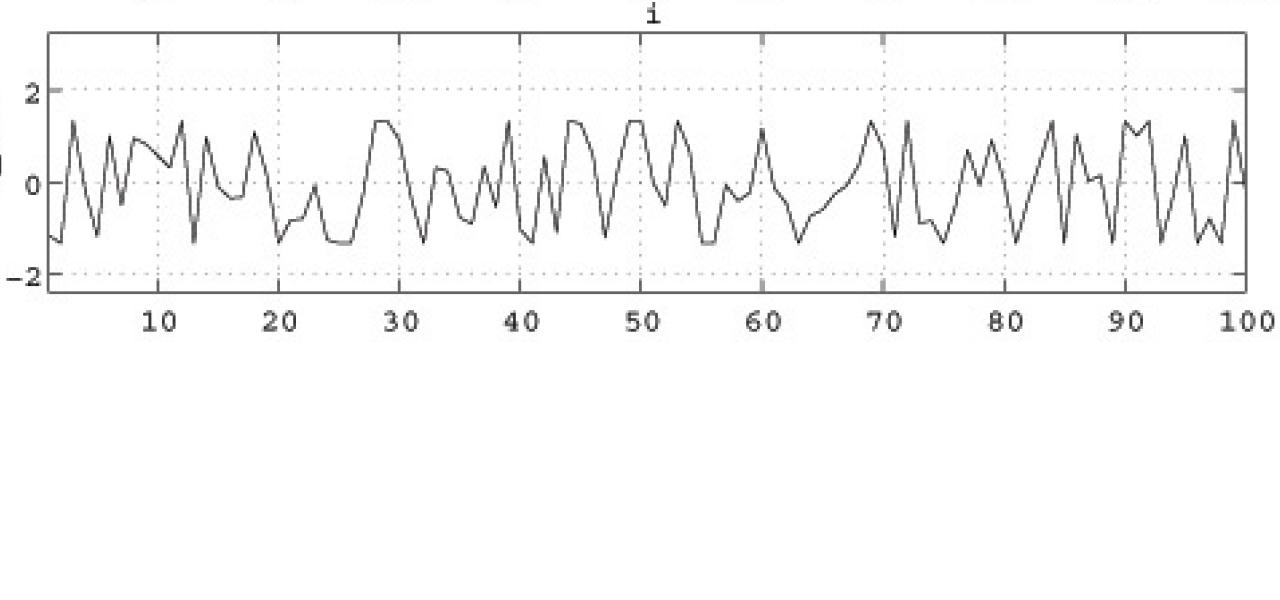
\includegraphics[scale=0.3]{residus.jpg}
    \end{center}

    \begin{solution}
      Le vecteur $b \notin \mathcal{C}(A) $ si et seulement si le nombre de
      contraintes est strictement supérieur au nombre de variables
      (en faisant l'hypothèse que les contraintes
      sont linéairement indépendantes).
      Pour plus d'explications, voir transparents CM 3.
    \end{solution}

  \item Vrai ou faux? Justifiez vos choix par quelques lignes, un contre-exemple ou un dessin. Soyez assez précis pour convaincre
    que vous ne devinez pas la réponse mais ne fournissez toutefois pas une justification formelle et détaillée.

    \begin{enumerate}

% polyhedron

      \item L'union de deux polyèdres est un polyèdre.

%\item The empty set is a polyhedron.

%extreme points

      \item Tout polyèdre $P$ peut être écrit sous forme géométrique $P=\{ {\bf x} \in {\bf R}^n: \bf A \bf x\geq \bf b\}$.

      \item Tout polyèdre $P$ peut être écrit sous forme standard
        $P=\{ {\bf x} \in {\bf R}^n: \bf A \bf x= \bf b, \bf x \geq 0\}$.


% \item L'ensemble $\{(x,y,z):x^2+y^2+z^2\leq 1\}$ est un polyèdre.

%\item A polyhedron in standard form always has an extreme point.

%\item A non-empty bounded polyhedra has at least one
%non-degenerate vertex.

%\item A point in a polyhedron in standard form can be expressed as
%a convex combination of the polyhedron vertices.

%\item Let $x_0$ and $x_1$ be two vertices of a polyhedron in ${\bf
%R}^n$ and let the polyhedron be defined by $m$ linear
%inequalities. Then here is a path from $x_0$ to $x_1$ along edges
%of the polyhedron that passes through at most $m^m$ edges.

%\item If there exists a vector $\bf q \neq \bf 0$ for which $\bf A
%\bf q=\bf 0$, then the polyhedron $\{\bf x: \bf A \bf x\geq \bf
%b\}$ doesn't have any vertex.

%\item Suppose that the polyhedron $\{{\bf x}: \bf A \bf x\geq \bf
%b\}$  is non-empty and bounded, then $\bf x = \bf 0$ is the only
%vector for which $\bf A \bf x = \bf 0$.

% solutions

      \item L'ensemble des solutions optimales d'un problème d'optimisation linéaire est un polyèdre.

%Consider the set $Q$ of optimal solutions to $\min \{ {\bf c}'
%{\bf x}: {\bf A} {\bf x} \geq {\bf b}, {\bf x} \in {\bf R}^n\}$.
%The set $Q$ is a polyhedron and its extreme points are extreme
%points of the polyhedron $\{{\bf x} \in {\bf R}^n: \bf A \bf x
%\geq \bf b\}$.

%\item A linear optimization problem may have exactly two optimal
%solutions.


%\item At an optimal solution of a linear optimization problem in
%${\bf R}^n$ there are $n$ active constraints.

      \item En toute solution optimale d'un problème d'optimisation linéaire de
        $n$ variables il y a au moins $n$  contraintes actives.


%\item Let $\bf x$ be a basic feasible solution associated with
%some basic matrix. If $\bf x$ is the unique optimal solution, then
%the reduced cost of every nonbasic variable is positive.

% simplex




%\item If a linear optimization problem has an unbounded optimal
%cost, then its dual is infeasible.


%\item If a linear optimization problem is infeasible, then its
%dual has unbounded optimal cost.


%\item L'optimisation linéaire permet de faire une régression linéaire minimisant la norme $||\cdot||_\infty$ des résidus.


    \end{enumerate}

    \begin{solution}
      \begin{enumerate}
        \item Faux, on sait qu'un polyèdre est convexe or
          $\{x | x \leq -1\} \cap \{x | x \geq 1\}$ n'est pas convexe.
        \item Vrai, c'est même sa définition.
        \item Faux, on sait qu'un polyèdre sous forme standard admet
          toujours un sommet alors qu'en général un polyèdre n'admet pas
          toujours un sommet.
          Par exemple, $\{(x_1,x_2) \in \R^2 | x_1 \geq 0\}$ n'admet
          pas de sommet. Il en pourra donc pas être écrit sous forme standard
          sans faire un changement de variable qui modifiera le polyèdre.
          Il ne faut d'ailleurs pas confondre ça avec le fait que tout
          problème d'optimisation linéaire peut s'écrire sous forme standard.
          Car ici, on accepte pas de changement de variable car ça
          modifie le polyèdre.
        \item Vrai. En effet, on ait que l'ensemble admissible $\mathcal{D}$
          est un polyèdre.
          L'ensemble des solutions qui ont un coût optimal
          \[ \{x | c^T x = z^*\} =
          \{x | c^T x \geq z^* \land (-c^T) x \geq -z^*\} \]
          est aussi un polyèdre.
          L'ensemble des solutions optimale est l'intersection des deux est
          donc aussi un polyèdre car l'intersection de deux polyèdres est
          un polyèdre.
        \item Faux.
          Il ne faut pas faire dire au théorème fondamental
          ce qu'il ne dit pas.
          Si l'ensemble admissible possède un sommet et que le coût
          optimal est fini,
          il \emph{existe} un sommet optimal mais
          toutes les solutions optimales ne sont
          pas spécialement des sommets.
          Par exemple, pour le problème d'optimisation linéaire suivant
          \begin{align*}
            \min x_1\\
            (x_1,x_2) & \geq 0
          \end{align*}
          la solution optimale $(0,0)$ est un sommet mais la solution
          optimale $(0,1)$
          n'en est pas une.
          $(0,1)$ serre d'ailleurs une seule contrainte,
          ce qui constitue un contre exemple car on a deux variables.
      \end{enumerate}
    \end{solution}

\end{enumerate}


\newpage

%******************************************************************************

\section{Méthode du simplexe}

\begin{enumerate}

  \item Soit le problème d'optimisation

    $
    \begin{array}{lrcr}
      \mini & -2x_1 - x_2 \\
      & x_1 - x_2 & \leq & 2\\
      & x_1 +  x_2 & \leq & 6\\
      & x_1, x_2 & \geq & 0
    \end{array}
    $

    Convertissez ce problème sous forme standard et trouvez un sommet pour
    lequel $x_1 = x_2 =0$.
    Résolvez le problème au moyen de la méthode
    du simplexe.
    Tracez une représentation graphique en terme des variables
    $x_1, x_2$ et indiquez le chemin suivi par la méthode.

    \begin{solution}
      En introduisant les variables d'écart $x_3$ et $x_4$,
      le tableau simplexe devient
      \[
        \begin{array}{cccc|l}
          -2 & -1 & 0 & 0 & z\\
          \hline
           1 & -1 & 1 & 0 & 2\\
           1 &  1 & 0 & 1 & 6
        \end{array}
      \]
      Le sommet $(0,0,2,6)$ n'est pas optimal car les coûts réduits
      $\tilde{c}_1 = -2$ et $\tilde{c}_2 = -1$ sont négatifs.
      Faisons rentrer $x_1$ dans la base (bien qu'on aurait tout autant
      pu faire rentrer $x_2$).
      Regardons qui on doit sortir de la base pour garder un sommet
      admissible.
      Si $x_1 = \lambda > 0$, on a $x = (\lambda, 0, 2-\lambda,6-\lambda)$.
      Si on voulait faire sortir, $x_4$, on aurait eu $x_4=0$ et
      donc $\lambda = 6$ et $x_3 = -4$ ce qui n'est pas admissible.
      C'est donc $x_3$ qui sort de la base.
      Le tableau simplexe devient alors
      \[
        \begin{array}{cccc|l}
          0 & -3 &  2 & 0 & z+4\\
          \hline
          1 & -1 &  1 & 0 & 2\\
          0 &  2 & -1 & 1 & 4
        \end{array}
      \]
      Le sommet $(2,0,0,4)$ n'est pas non plus optimal car le coût
      réduit $\tilde{c}_2 = -1$ est négatif.
      Faisons donc rentrer $x_2$ dans la base car c'est lui qui a un
      coût réduit négatif.
      À nouveau, on a $x = (2+\lambda,\lambda,0,4-2\lambda)$.
      Comme $\lambda > 0$, $x_1$ ne peut pas être nul.
      C'est donc $x_4$ qui sort de la base.
      \[
        \begin{array}{cccc|l}
          0 & 0 &  1/2 & 3/2 & z+10\\
          \hline
          1 & 0 &  1/2 & 1/2 & 4\\
          0 & 1 & -1/2 & 1/2 & 2
        \end{array}
      \]
      Les coût réduits $\tilde{c}_3$ et $\tilde{c}_4$ sont négatifs,
      le sommet $(4,2,0,0)$ est donc optimal.
      On a donc $\xopt = (4,2,0,0)$ avec $z^* = -10$.
    \end{solution}

  \item Considérez le problème

    $
    \begin{array}{llcr}
      \mini & 20 x_1+\alpha x_2+12 x_3\\
      & x_1  & \leq & 400\\
      &2x_1+\beta x_2+x_3 & \leq & 1000\\
      &2x_1+\gamma x_2+ 3x_3 & \leq & 1600\\
      & x_1, x_2, x_3 & \geq & 0
    \end{array}
    $

    Proposez, si possible,
    des valeurs pour $\alpha, \beta$ et $\gamma$ pour lesquelles:

    \begin{enumerate}

      \item Le coût optimal est fini et la solution optimale est unique.

      \item Le coût optimal est fini
        et il y a une infinité de solutions optimales.

      \item Le coût optimal est non borné
        (trouvez une paramétrisation de valeurs de $x$
        parmi lesquelles se trouvent des solutions de coûts
        arbitrairement faibles).

      \item Le poly\`edre possède un sommet dégénéré.

    \end{enumerate}

    \begin{solution}
      En introduisant les variables d'écart $x_4$, $x_5$ et $x_6$,
      le tableau simplexe devient
      \[
        \begin{array}{cccccc|l}
          20 & \alpha & 12 & 0 & 0 & 0 & z\\
          \hline
           1 & 0      &  0 & 1 & 0 & 0 & 400\\
           2 & \beta  &  1 & 0 & 1 & 0 & 1000\\
           2 & \gamma &  3 & 0 & 0 & 1 & 1600
        \end{array}
      \]
      \begin{enumerate}
        \item Si $\alpha > 0$, $(0,0,0)$ est l'unique sommet optimal.
          En effet, il est impossible d'avoir $z^* = 0$ avec d'autres sommets.
        \item Si $\alpha = 0$, $(0,x_2,0)$ est optimal pour tout $x_2$
          tel que la solution est admissible.
        \item Si $\alpha < 0$ et $\beta,\gamma \leq 0$.
          $(0,\lambda,0)$ est admissible pour tout $\lambda > 0$ et
          $z^*$ est aussi petit que l'on veut.
        \item Pour avoir un sommet dégénéré, il faut qu'un terme indépendant
          vaille 0.
          En sortant $x_2$ de la base et en y fesant rentrer $x_3$, on
          optient le tableau simplexe suivant (si $\beta \neq 0$)
          \[
            \begin{array}{cccccc|l}
              20 & \alpha & 12 & 0 & 0 & 0 & z\\
              \hline
              1 & 0      &  0 & 1 & 0 & 0 & 400\\
              2 & \beta  &  1 & 0 & 1 & 0 & 1000\\
              2-2\frac{\gamma}{\beta} & 0
              & 3-\frac{\gamma}{\beta} & 0 & -\frac{\gamma}{\beta} & 1
              & 1600 - 1000\frac{\gamma}{\beta}
            \end{array}
          \]
          Un choix possible est donc $(\beta,\gamma) = (1000,1600)$
          qui aurait comme sommet dégénéré $(0,1,0)$.
      \end{enumerate}
    \end{solution}

  \item
    Résoudre par l'algorithme du simplexe les problèmes
    \begin{enumerate}
      \item
        $
        \begin{array}{llcr}
          \maxi & 2x_1+3x_2\\
                & x_1+2x_2 & \leq & 4\\
                & x_1+x_2 & = & 3\\
                & x_1, x_2& \geq & 0
        \end{array}
        $
      \item
        $
        \begin{array}{llcr}
          \maxi & 20 x_1+16x_2+12 x_3\\
                & x_1  & \leq & 400\\
                &2x_1+x_2+x_3 & \leq & 1000\\
                &2x_1+2x_2+ 3x_3 & \leq & 1600\\
                & x_1, x_2, x_3 & \geq & 0
        \end{array}
        $
      \item
        $
        \begin{array}{llcr}
          \maxi & 4x_1+3x_2+6x_3\\
                & 3x_1+x_2+3x_3 & \leq & 30\\
                & 2x_1+2x_2+3x_3 & \leq & 40\\
                & x_1, x_2, x_3 & \geq & 0
        \end{array}
        $
      \item
        $
        \begin{array}{llcr}
          \maxi & -x_1+4x_2\\
                & -3x_1+4x_2 & \leq & 6\\
                & x_1+2x_2 & \leq & 4\\
                & x_2& \geq & -3
        \end{array}
        $
    \end{enumerate}

    \begin{solution}
      \begin{enumerate}
        \item En mettant le problème sous forme standard,
          on obtient le tableau simplexe suivant
          \[
            \begin{array}{ccc|l}
              -2 & -3 & 0 & -z\\
              \hline
              0 &  1 & 1 & 1\\
              1 &  1 & 0 & 3\\
            \end{array}
          \]
          on peut facilement trouver un sommet sans devoir passer
          par le problème annexe.
          On trouve
          \[
            \begin{array}{ccc|l}
              0 & -1 & 0 & -z+6\\
              \hline
              0 &  1 & 1 & 1\\
              1 &  1 & 0 & 3\\
            \end{array}
          \]
          En faisant rentrer $x_2$ dans la base,
          on doit faire sortir $x_3$.
          On a alors
          \[
            \begin{array}
              {ccc|l}
              0 & -1 & 0 & -z+7\\
              \hline
              0 &  1 & 1 & 1\\
              1 &  1 & 0 & 3\\
            \end{array}
          \]
          Dès lors, $\xopt = (2,1,0)$ et $z^* = 7$.
        \item
          \label{itm:sim400}
          Le tableau simplexe est le suivant
          \[
            \begin{array}{cccccc|l}
              -20 & -16 & -12 & 0 & 0 & 0 & -z\\
              \hline
              1 &   0 &   0 & 1 & 0 & 0 & 400\\
              2 &   1 &   1 & 0 & 1 & 0 & 1000\\
              2 &   2 &   3 & 0 & 0 & 1 & 1600
            \end{array}
          \]

          En faisant renter $x_1$ dans la base,
          on voit qu'on doit faire sortir $x_4$.
          On a donc
          \[
            \begin{array}{cccccc|l}
              0 & -16 & -12 & 20 & 0 & 0 & -z+8000\\
              \hline
              1 &   0 &   0 &  1 & 0 & 0 & 400\\
              0 &   1 &   1 & -2 & 1 & 0 & 200\\
              0 &   2 &   3 & -2 & 0 & 1 & 800
            \end{array}
          \]

          Faisons maintenant rentrer $x_2$ dans la base en faisant sortir $x_5$
          \[
            \begin{array}{cccccc|l}
              0 & 0 & 4 & -12 & 16 & 0 & -z+11200\\
              \hline
              1 & 0 & 0 &   1 &  0 & 0 & 400\\
              0 & 1 & 1 &  -2 &  1 & 0 & 200\\
              0 & 0 & 1 &   2 & -2 & 1 & 400
            \end{array}
          \]

          Essayons maintenant en faisant rentre $x_4$.
          On doit alors sortir $x_6$.
          \[
            \begin{array}{cccccc|l}
              0 & 0 &  10  & 0 &  4 &  6   & -z+13600\\
              \hline
              1 & 0 & -1/2 & 0 &  1 & -1/2 & 200\\
              0 & 1 &  2   & 0 & -1 &  1   & 600\\
              0 & 0 &  1/2 & 1 & -1 &  1/2 & 200
            \end{array}
          \]
          La solution optimale est donc $x^* = (200,600,0)$ avec $z^* = 13600$.
        \item
          On a le tableau simplexe suivant
          \[
            \begin{array}{ccccc|l}
              -4 & -3 & -6 & 0 & 0 & -z\\
              \hline
               3 &  1 &  3 & 1 & 0 & 30\\
               2 &  2 &  3 & 0 & 1 & 40\\
            \end{array}
          \]

          En faisant rentrer $x_3$ dans la base,
          $x_4$ doit sortir, ce qui donne
          \[
            \begin{array}{ccccc|l}
               2 & -1   & 0 & 2   & 0 & -z+60\\
              \hline
               1 &  1/3 & 1 & 1/3 & 0 & 10\\
              -1 &  1   & 0 & -1  & 1 & 10\\
            \end{array}
          \]

          Faisons maintenant rentrer $x_2$ et donc sortir $x_5$
          \[
            \begin{array}{ccccc|l}
               1   & 0 & 0 &  1   &  1   & -z+70\\
              \hline
               4/3 & 0 & 1 &  2/3 & -1/3 & 20/3\\
              -1   & 1 & 0 & -1   &  1   & 10\\
            \end{array}
          \]
          d'où la solution optimale $\xopt = (0,10,\frac{20}{3})$
          de coût optimal $z^* = 70$.
        \item
          Faisons les changements de variables $x_1 = x_3 - x_4$ et
          $x_2 = x_5-3$.
          Le problème devient alors
          \begin{align*}
            -12 - \min x_3 - x_4 - 4x_5\\
            -3x_3 + 3x_4 + 4x_5 & \leq 18\\
            x_3 - x_4 + 2x_5 & \leq 10\\
            x_3,x_4,x_5 & \geq 0.
          \end{align*}
          En ajoutant les variables d'écart nécessaire,
          on a le tableau simplexe
          \[
            \begin{array}{ccccc|l}
              1 & -1 & -4 & 0 & 0 & -z-12\\
              \hline
              -3 & 3 & 4 & 1 & 0 & 18\\
              1 & -1 & 2 & 0 & 1 & 10\\
            \end{array}
          \]

          En ajoutant $x_5$ à la base, on doit retirer $x_6$.
          On a alors
          \[
            \begin{array}{ccccc|l}
              -2 & 2 & 0 & 1 & 0 & -z+6\\
              \hline
              -3/4 & 3/4 & 1 & 1/4 & 0 & 9/2\\
              5/2 & -5/2 & 0 & -1/2 & 1 & 1\\
            \end{array}
          \]

          Ajoutons maintenant $x_3$ à la base. $x_7$ doit alors sortir
          \[
            \begin{array}{ccccc|l}
              0 &  0 & 0 &  3/5  & 4/5  & -z+34/5\\
              \hline
              0 &  0 & 1 &  1/10 & 3/10 & 24/5\\
              1 & -1 & 0 & -1/5  & 2/5  & 2/5\\
            \end{array}
          \]

          On a donc $(x_3,x_4,x_5) = \frac{1}{5}(2,0,24)$ d'où
          $\xopt = \frac{1}{5}(2, 9)$ avec un coût optimal
          $z^* = \frac{34}{5}$.
      \end{enumerate}
    \end{solution}

  \item Nous reprenons un des problèmes précédents.
    Un étudiant dispose de 100 heures de travail pour
    étudier les examens A, B et C.
    Il pense gagner par heure de travail sur chaque cours 1/5 de points pour
    le cours A, 2/5 de points pour le cours B et 3/5 pour le cours C.
    Chaque examen est coté sur 20.
    Les exercices de ces cours comptent pour la moitié de la cote finale.
    Ses résultats pour les exercices lui ont été communiqués.
    Il a obtenu 12/20 pour A, 12.5/20 pour B et 13.4/20 pour C.
    L'étudiant doit obtenir au minimum une cote globale de 10/20 pour chaque
    cours.
    Tous les cours ont la même pondération et l'étudiant désire obtenir la
    moyenne la plus élevée possible.

    Formulez ce problème comme un problème d'optimisation linéaire  et résolvez-le.
    Vous pouvez utiliser le fait que l'étudiant a avantage à utiliser la
    totalité des 100 heures de travail.
    L'étudiant obtiendra-t-il une distinction?

    \begin{solution}
      Soient $x_A$, $x_B$ et $x_C$, respectivement
      le nombre d'heures étudiées pour $A$, $B$ et $C$.
      Le nombres d'heures optimaux sont les solutions du problème
      d'optimisation suivant
      \begin{align*}
        \max x_A + 2x_B + 3x_C\\
        x_A & \leq 100\\
        x_A & \geq 40\\
        x_B & \leq 50\\
        x_B & \geq 18.75\\
        x_C & \leq 100/3\\
        x_C & \geq 11\\
        x_A + x_B + x_C & = 100
      \end{align*}
      En posant $x_1,x_2,x_3$ le nombre d'heures étudiées pour faire plus
      que 10, c'est à dire
      \begin{align*}
        x_A & = 40 + x_1\\
        x_B & = 18.75 + x_2\\
        x_C & = 11 + x_3
      \end{align*}

      On sait que les $x_1,x_2,x_3$ donnant les $x_A,x_B,x_C$ optimaux
      sont solutions du problème d'optimisation suivant.
      \begin{align*}
        \max x_1 + 2x_2 + 3x_3\\
        x_A & \leq 60\\
        x_B & \leq 31.25\\
        x_C & \leq 67/3\\
        x_A + x_B + x_C & = 30.25\\
        x & \geq 0
      \end{align*}

      Le tableau simplexe est alors
      \[
        \begin{array}{cccccc|l}
          -1 & -2 & -3 & 0 & 0 & 0 & -z\\
          \hline
          1 & 0 & 0 & 1 & 0 & 0 & 60\\
          0 & 1 & 0 & 0 & 1 & 0 & 31.25\\
          0 & 0 & 1 & 0 & 0 & 1 & 67/3\\
          1 & 1 & 1 & 0 & 0 & 0 & 30.25
        \end{array}
      \]

      Il y a 4 contraintes mais que 3 variables de base, il en manque donc
      une pour faire un sommet.
      On peut cependant facilement ajouter $x_1$ dans la base
      car $60-30.25 > 0$ ou $x_2$ car $31.25-30.25 >0 $.
      Il n'y a donc pas besoin de passer par le problème annexe pour trouver
      un sommet de départ.
      Faisons rentrer $x_2$
      \[
        \begin{array}{cccccc|l}
           1 & 0 & -1 & 0 & 0 & 0 & -z + 61\\
          \hline
           1 & 0 &  0 & 1 & 0 & 0 & 60\\
          -1 & 0 & -1 & 0 & 1 & 0 & 1\\
           0 & 0 &  1 & 0 & 0 & 1 & 67/3\\
           1 & 1 &  1 & 0 & 0 & 0 & 30.25
        \end{array}
      \]

      Faisons maintenant rentrer $x_3$, pour cela, on doit faire sortir $x_6$
      \[
        \begin{array}{cccccc|l}
           1 & 0 & 0 & 0 & 0 &  1 & -z + 250/3\\
          \hline
           1 & 0 & 0 & 1 & 0 &  0 & 60\\
          -1 & 0 & 0 & 0 & 1 &  1 & 70/3\\
           0 & 0 & 1 & 0 & 0 &  1 & 67/3\\
           1 & 1 & 0 & 0 & 0 & -1 & 95/12
        \end{array}
      \]

      On trouve donc $(x_1,x_2,x_3) = (0,95/12,67/3)$ d'où
      \[ (x_A^*,x_B^*,x_C^*) = (40,80/3,100/3). \]
      Il aura donc $10$ pour A, $11.58\bar{3}$ pour B et $20$ pour C
      ce qui lui fait une moyenne de $13.86\bar{1}$ ou encore
      $69.30\bar{5}\,\%$.
      Il aura donc une distinction car la barre est à $68\,\%$.
    \end{solution}

  \item Une société produit des biens A, B et C.
    La production des biens nécessite l'utilisation de 4 machines.
    Les temps de production et les profits générés sont repris dans le tableau

    $
    \begin{array}{l|llll|l}
      & 1 & 2 & 3 & 4 & \mbox{profit}\\
      \hline
      A & 1 & 3 & 1 & 2 & 6\\
      B & 6 & 1 & 3 & 3 & 6\\
      C & 3 & 3 & 2 & 4 & 6
    \end{array}
    $
    \\

    Si les temps de production disponibles sur les machines 1, 2, 3 et 4  sont de 84, 42, 21 et 42,
    déterminez la quantité de biens à produire pour maximiser le profit.

    \begin{solution}
      Soit $x_i$ la quantité de biens $i$ produite.
      Le problème d'optimisation est donc le suivant
      \begin{align*}
        -\min -x_A - x_B - x_C\\
         x_A + 6x_B + 3x_C & \leq 84\\
        3x_A +  x_B + 3x_C & \leq 42\\
         x_A + 3x_B + 2x_C & \leq 21\\
        2x_A + 3x_B + 4x_C & \leq 42\\
        x & \geq 0.
      \end{align*}
      En introduisant les variables d'écart nécessaire,
      on obtient le tableau simplexe suivant
      \[
        \begin{array}{ccccccc|l}
          -6 & -6 & -6 & 0 & 0 & 0 & 0 & -z\\
          \hline
           1 &  6 &  3 & 1 & 0 & 0 & 0 & 84\\
           3 &  1 &  3 & 0 & 1 & 0 & 0 & 42\\
           1 &  3 &  2 & 0 & 0 & 1 & 0 & 21\\
           2 &  3 &  4 & 0 & 0 & 0 & 1 & 42\\
        \end{array}
      \]
      En faisant rentrer $x_1$, on obtient
      \[
        \begin{array}{ccccccc|l}
          0 & -4   & 0 & 0 &  2   & 0 & 0 & -z+84\\
          \hline
          0 & 17/3 & 2 & 1 & -1/3 & 0 & 0 & 70\\
          1 &  1/3 & 1 & 0 &  1/3 & 0 & 0 & 14\\
          0 &  8/3 & 1 & 0 & -1/3 & 1 & 0 & 7\\
          0 &  7/3 & 2 & 0 & -2/3 & 0 & 1 & 14\\
        \end{array}
      \]
      Rentrons maintenant $x_2$ dans la base pour obtenir
      \[
        \begin{array}{ccccccc|l}
          0 & 0 &  3/2 & 0 &  3/2  &   3/2 & 0 & -z+189/2\\
          \hline
          0 & 0 & -1/8 & 1 &  9/24 & -17/8 & 0 & 441/8\\
          1 & 0 &  7/8 & 0 &  9/24 &  -3/8 & 0 & 105/8\\
          0 & 1 &  3/8 & 0 & -1/8  &   3/8 & 0 & 21/8\\
          0 & 0 &  9/8 & 0 & -9/24 &  -7/8 & 1 & 63/8\\
        \end{array}
      \]
      Le sommet optimal est donc $x^* = \frac{1}{8}(105,21,0)$ avec comme
      coût optimal $z^* = 189/2$.
    \end{solution}

  \item Résoudre par la méthode du simplexe en utilisant la règle de Bland

    $
    \begin{array}{llcr}
      \maxi & 10 x_1-57 x_2-9x_3-24x_4\\
      & 0.5x_1-5.5x_2-2.5x_3+9x_4 & \leq & 0\\
      & 0.5x_1-1.5x_2-0.5x_3+x_4 & \leq & 0\\
      & x_1 & \leq &1\\
      & x_1, x_2, x_3, x_4 & \geq & 0
    \end{array}
    $


    \begin{solution}
      La règle de Bland consiste à choisir la variable $x_r$ de plus petit
      indice $r$ parmi les variables candidates à l'entrée $i = 1,2, \dots, n$
      (idem pour les variables candidates à la sortie).

      Ça permet d'éviter qu'on boucle infiniment sur des sommets
      dégénérés de même coût dans l'algorithme du simplexe.

      On a donc
      \[
        \begin{array}{ccccccc|l}
          -10 & 57   & 9    & 24 & 0 & 0 & 0 & -z\\
          \hline
          0.5 & -5.5 & -2.5 &  9 & 1 & 0 & 0 & 0\\
          0.5 & -1.5 & -0.5 &  1 & 0 & 1 & 0 & 0\\
          1   &  0   &  0   &  0 & 0 & 0 & 1 & 1
        \end{array}
      \]

      Faisons rentrer $x_1$ dans la base.
      On a le choix entre faire sortir $x_5$ et $x_6$.
      La règle de Bland nous impose de faire sortir $x_5$.
      \[
        \begin{array}{ccccccc|l}
          0 & -53 & -41 & 204 & 20 & 0 & 0 & -z\\
          \hline
          1 & -11 &  -5 &  18 &  2 & 0 & 0 & 0\\
          0 &   4 &   2 &  -8 &  0 & 1 & 0 & 0\\
          0 &  11 &   5 & -18 & -2 & 0 & 1 & 1
        \end{array}
      \]

      Faisons maintenant rentrer $x_2$.
      On doit donc faire sortir $x_6$.
      \[
        \begin{array}{ccccccc|l}
          0 & 0 & -29/2 & 98 & 20 &  53/4 & 0 & -z\\
          \hline
          1 & 0 &   1/2 & -4 &  2 &  11/4 & 0 & 0\\
          0 & 1 &   1/2 & -2 &  0 &   1/4 & 0 & 0\\
          0 & 0 &  -1/2 &  4 & -2 & -11/4 & 1 & 1
        \end{array}
      \]

      On doit maintenant faire rentrer $x_3$.
      On a le choix entre faire sortir $x_1$ ou $x_2$ mais la
      règle de Bland nous impose de sortir $x_1$.
      \[
        \begin{array}{ccccccc|l}
          29 & 0 & 0 & -18 & 78 & 93   & 0 & -z\\
          \hline
           1 & 0 & 1 &  -8 &  4 & 11/4 & 0 & 0\\
          -1 & 1 & 0 &   2 & -2 & -5/4 & 0 & 0\\
           1 & 0 & 0 &   0 &  0 &  0   & 1 & 1
        \end{array}
      \]

      On doit alors faire rentrer $x_4$ et pour cela faire sortir
      $x_2$.
      \[
        \begin{array}{ccccccc|l}
          20   & 9   & 0 & 0 & 60   & 141/2 & 0 & -z\\
          \hline
          -3   & 4   & 1 & 0 & -4   & -9/2  & 0 & 0\\
          -1/2 & 1/2 & 0 & 1 & -1/2 & -5/4  & 0 & 0\\
           1   & 0   & 0 & 0 &  0   &  0    & 1 & 1
        \end{array}
      \]

      $(0,0,0,0)$ est donc assurément un sommet optimal.
      Mais comme le coût n'a jamais changé, tous les sommets
      étaient optimaux.

    \end{solution}

  \item Proposez une méthode de recherche d'un sommet du polyhèdre

    $
    \begin{array}{lrcr}
      & 2x_1-3x_2 +2x_3 & \geq & 3\\
      & -x_1+x_2 +x_3 & \geq & 5\\
      & x_1, x_2, x_3 & \geq & 0
    \end{array}
    $

    \begin{solution}
      Commençons par écrire le polyèdre sous forme standard

      \begin{align*}
        2x_1 - 3x_2 + 2x_3 - x_4 & = 3\\
        -x_1 +  x_2 +  x_3 - x_5 & = 5\\
         x_1, x_2, x_3, x_4, x_5 & \geq 0
      \end{align*}

      Il n'est pas facile de deviner un sommet immédiatement car en
      prenant comme base $x_4,x_5$, on arrive à $(x_4,x_5)=(-3,-5)$
      qui n'est pas admissible.

      On fait donc appel au problème annexe
      \begin{align*}
        \min \sum_i y_i\\
        Ax + y & = b\\
        x,y & \geq 0.
      \end{align*}

      Si le coût optimal du problème annexe est non-nul,
      c'est que le polyèdre ne possède pas de sommet.
      Sinon, $(x_1^*, x_2^*, x_3^*)$ forme un sommet optimal.
      On résoud donc le problème annexe avec le simplexe.
      Le tableau simplexe est

      \[
        \begin{array}{ccccccc|l}
           0 &  0 & 0 &  0 &  0 & 1 & 1 & z\\
          \hline
           2 & -3 & 2 & -1 &  0 & 1 & 0 & 3\\
          -1 &  1 & 1 &  0 & -1 & 0 & 1 & 5\\
        \end{array}
      \]

      L'avantage du problème annexe c'est qu'on peut trouver immédiatement
      un sommet pour commencer l'algorithme du simplexe
      si on avait $b \geq 0$.
      Il suffit de prendre $y$ comme base.
      En effet, $x = (0,0,0,0,0,3,5)$ est un sommet de ce polyèdre annexe.
      Bien qu'on ne demande qu'une méthode de recherche,
      notre curiosité nous impose de continuer la résolution,
      on obtient alors le tableau simplexe

      \[
        \begin{array}{ccccccc|l}
          -1 &  2 & -3 &  1 &  1 & 0 & 0 & z-8\\
          \hline
           2 & -3 &  2 & -1 &  0 & 1 & 0 & 3\\
          -1 &  1 &  1 &  0 & -1 & 0 & 1 & 5\\
        \end{array}
      \]

      On peut faire rentrer $x_3$ dans la base,
      on obtient alors

      \[
        \begin{array}{ccccccc|l}
           2 & -5/2 &  0 & -1/2 &  1 &  3/2 & 0 & z-7/2\\
          \hline
           1 & -3/2 &  1 & -1/2 &  0 &  1/2 & 0 & 3/2\\
          -2 &  5/2 &  0 &  1/2 & -1 & -1/2 & 1 & 7/2\\
        \end{array}
      \]

      On voit qu'on s'approche de $z = 0$ mais on y est pas encore.
      D'ailleurs il reste des coûts réduits négatifs, faisons maintenant
      rentrer $x_2$ dans la base, on obtient

      \[
        \begin{array}{ccccccc|l}
           0   &  0   &  0 &  0   &  0   &  1   & 1   & z\\
          \hline
          -1/5 &  0   &  1 & -1/5 & -3/5 &  1/5 & 3/5 & 18/5\\
          -4/5 &  1   &  0 &  1/5 & -2/5 & -1/5 & 2/5 &  7/5\\
        \end{array}
      \]

      On a maintanenant bien $z = 0$.
      Notre polyèdre avait donc au moins un sommet.
      $\frac{1}{5}(0,7,18)$ est un de ces sommets.
    \end{solution}

  \item  Considérez le problème d'optimisation

    $
    \begin{array}{llcr}
      \mini & 20 x_1+\alpha x_2+12 x_3\\
      & x_1  & \leq & 4\\
      &2x_1 - x_2+x_3 & \leq & 10\\
      &2x_1+\beta x_2+ 3x_3 & \leq & 16\\
      & x_1, x_2, x_3 & \geq & 0
    \end{array}
    $

    Trouvez une solution optimale au moyen de l'algorithme du simplexe
    lorsque $\alpha = -2$ et $\beta = 1$.
    Proposez des valeurs pour $\alpha$ et $\beta$ pour lesquelles
    le coût optimal est non borné et
    proposez dans ce cas une solution pour laquelle le coût
    optimal est inférieur à $-1000$.
    % FIXME: ne serait-ce pas mieux de dire "solution ADMISSIBLE"
    %        car solution est défini comme n'importe quel x

    \begin{solution}
      Pour $\alpha = -2$ et $\beta = 1$, le tableau simplexe est
      \[
        \begin{array}{cccccc|l}
          20 & -2 & 12 & 0 & 0 & 0 & z\\
          \hline
          1  &  0 &  0 & 1 & 0 & 0 & 4\\
          2  & -1 &  1 & 0 & 1 & 0 & 10\\
          2  &  1 &  3 & 0 & 0 & 1 & 16\\
        \end{array}
      \]
      en ajoutant $x_2$ à la base,
      il faut retirer $x_6$, on a alors
      \[
        \begin{array}{cccccc|l}
          24 & 0 & 18 & 0 & 0 & 2 & z+32\\
          \hline
          1  & 0 &  0 & 1 & 0 & 0 & 4\\
          4  & 0 &  4 & 0 & 1 & 1 & 26\\
          2  & 1 &  3 & 0 & 0 & 1 & 16\\
        \end{array}
      \]
      La solution optimale vaut donc $\xopt = (0,16,0)$ avec
      un coût optimal de $-32$.

      Pour que le coût soit non-borné, il suffit que $\alpha < 0$ et que
      $\beta \leq 0$.
      Prenons $(\alpha,\beta) = (-1,-1)$.
      On remarque alors que $(0,1001,0)$ est admissible et que son
      coût $-1001$ est inférieur à $-1000$.
    \end{solution}

  \item  Considérez le problème d'optimisation

    $
    \begin{array}{llcr}
      \maxi
      & \alpha x_1 + 16x_2+ 12x_3\\
      &        x_1                & \leq & 400\\
      &       2x_1 +   x_2+   x_3 & \leq & 1000\\
      &       2x_1 +  2x_2+  3x_3 & \leq & 1600\\
      &        x_1, x_2, x_3 & \geq & 0
    \end{array}
    $

    Trouvez une solution optimale au moyen de l'algorithme du simplexe
    lorsque $\alpha=20$.
    Existe-t-il une valeur de $\alpha$ pour laquelle le coût optimal
    est non borné?
    Si oui,
    proposez une solution pour laquelle le coût est supérieur à 10000.
    Si non, justifiez votre réponse.

    \begin{solution}
      Pour la résolution du simplexe, voir l'exercice~\ref{itm:sim400}.

      Si le coût optimal est non borné,
      c'est qu'il existe une demi-droite incluse au domaine admissible
      au long de laquelle $x_1 + 16x_2 + 12x_3$ augmente.
      Seulement, on peut remarqué géométriquement que le domaine admissible
      est compacte.
      On peut aussi s'en sortir algébriquement en se disant que
      si le coût augmente à l'infini, c'est au moins une variable augmente
      à l'infini.
      En tenant compte des contraintes, comme tous les coefficients
      sont positifs, il faut qu'au moins une variable tende vers
      $-\infty$ ce qui est impossible car elles sont positive.
      Tout cela pour dire qu'il n'existe pas de valeur d'$\alpha$
      pour laquelle le coût optimal est non borné.
    \end{solution}

\end{enumerate}


\newpage

%******************************************************************************

\section{Dualité I: formulation, relations d'exclusion, solution}


{\bf Forme géométrique}

Problème primal

$
\begin{array}{lrcr}
  \mini & c^T x\\
  & A x & \geq &  b\\
  & x   & \geq & 0
\end{array}
$

Problème dual

$
\begin{array}{lrcr}
  \maxi & b^Ty\\
  & A^T y & \leq &  c\\
  & y   & \geq & 0
\end{array}
$\\


{\bf Forme standard}



Problème primal

$
\begin{array}{lrcr}
  \mini & c^T x\\
  & A x & = &  b\\
  & x   & \geq & 0
\end{array}
$



Problème dual


$
\begin{array}{lrcr}
  \maxi & b^T y\\
  & A^T y & \leq &  c
\end{array}
$


\newpage



\begin{enumerate}

  \item \label{e5.1} Trouvez le dual du problème

    $
    \begin{array}{llcr}
      \mini & 3x_1-9x_2\\
      & 2x_1-x_2+x_3 & \geq & 3\\
      & x_1-x_2 -3x_3 & \geq & 2\\
      & x_1, x_2, x_3 & \geq & 0
    \end{array}
    $

    \begin{solution}
      $
      \begin{array}{llcr}
        \maxi & 3y_1 + 2y_2\\
        & 2y_1 + y_2 & \leq & 3\\
        & -y_1 - y_2 & \leq & -9\\
        & y_1 - 3y_2 & \leq & 0\\
        & y & \geq & 0
      \end{array}
      $
    \end{solution}


  \item Trouvez le dual du problème

    $
    \begin{array}{llcr}
      \mini & 3x_1-9x_2\\
      & 4x_1-x_2+x_3 & = & 3\\
      & x_1-x_2 -6x_3 & \geq & 2\\
      & x_1-4x_2 -6x_3 & \leq & 8\\
      & x_1, x_2 & \geq & 0
    \end{array}
    $

    \begin{solution}
      $
      \begin{array}{lrcr}
        \maxi & 3y_1 + 2y_2 + 8y_3\\
        & 4y_1 + y_2 + y_3 & \leq & 3\\
        & -y_1 + -y_2 -4y_3 & \leq & 2\\
        & y_1 -6y_2 -6y_3 & = & 0\\
        & y_2 & \geq & 0\\
        & y_3 & \leq & 0

      \end{array}
      $
    \end{solution}


  \item Trouvez le dual du problème

    $
    \begin{array}{llcr}
      \mini & c^T x\\
      & a_1^T x& = & b_1\\
      & a_2^T  x & \geq & b_2\\
      & a_3^T x & \leq & b_3\\
      & x& \geq & 0
    \end{array}
    $

    \begin{solution}
      $
      \begin{array}{llcr}
        \maxi & b^T x\\
        & Ay & \leq & c\\
        & y_1 & & \text{libre}\\
        & y_2 & \geq & 0\\
        & y_3 & \leq & 0
      \end{array}
      $

      où $A = \begin{pmatrix}a_1 & a_2 & a_3\end{pmatrix}$
    \end{solution}

  \item Trouvez le dual du problème de trois variables

    $
    \begin{array}{llcr}
      \mini & c^T x\\
      & a^T x& = & b\\
      & x_1 &  & \mbox{libre}\\
      & x_2 & \geq & 0\\
      & x_3 & \leq & 0
    \end{array}
    $

    \begin{solution}
      $b$ est un scalaire

      $
      \begin{array}{llcr}
        \maxi & b y\\
        & a_1 y & = & c_1\\
        & a_2 y & \leq & c_2\\
        & a_3 y & \geq & c_3\\
        & y & & \text{libre}
      \end{array}
      $
    \end{solution}

  \item Trouvez une formulation duale du  problème

    $
    \begin{array}{lrcr}
      \mini & c^T x\\
      & A x & = &  b\\
      & x   & \geq & a
    \end{array}
    $

    où $a \geq 0$.

    \begin{solution}
      L'astuce ici est de prendre des nouvelles variables pour chacune des
      (in)équations.
      On réécrit donc le problème d'optimisation linéaire comme suit

      $
      \begin{array}{lrcr}
        \mini & c^T x\\
        & A x & = &  b\\
        & I x   & \geq & a\\
        & x & & \mbox{ libre}
      \end{array}
      $

      où le dual appairait plus clairement

      $
      \begin{array}{lrcr}
        \maxi & b^Ty_1+a^Ty_2\\
        & Ay_1 + Iy_2 & = & c\\
        & y_1 & & \text{libre}\\
        & y_2 & \geq & 0.
      \end{array}
      $

      Si $x$ était un vecteur, $y_1$ et $y_2$ seront des vecteurs également.

      On peut s'en sortir avec moins de variables $y_i$ en faisant
      le changement de variable $x' + a = x$, d'où

      $
      \begin{array}{lrcr}
        \mini & c^T x' + c^Ta\\
        & A x' & = &  b - Aa\\
        & x'   & \geq & 0.
      \end{array}
      $

      On peut retirer $c^Ta$ car c'est une constante.
      Le dual est alors

      $
      \begin{array}{lrcr}
        \maxi & (b-Aa)^Ty\\
        & A^Ty & \leq & c
      \end{array}
      $

      \textbf{TODO} comment utilise-t-on le fait que $a \geq 0$ ?

      \textbf{TODO} ça a du sens de prendre le dual si on a fait un changement
      de variable ?
    \end{solution}

  \item Trouvez une formulation duale du  problème

    $
    \begin{array}{lrcrcrcr}
      \mini & c^T x\\
      & b_1 & \leq & A x & \leq &  b_2\\
      & x   & \geq & 0
    \end{array}
    $

    \begin{solution}
      $
      \begin{array}{lrcrcrcr}
        \maxi & b_{1}^{T}y_{1} + b_{2}^{T}y_{2}\\
        & A^{T}y_{1} & \leq & c\\
        & A^{T}y_{2} & \geq & c\\
        & y_1 & \geq & 0\\
        & y_2 & \leq & 0
      \end{array}
      $
    \end{solution}


  \item Comment résoudre le problème

    $
    \begin{array}{llcr}
      \mini & 50x_1+25x_2\\
      & x_1+3x_2 & \geq & 8\\
      & 3x_1+4x_2 & \geq & 19\\
      & 3x_1+x_2 & \geq & 7\\
      & x_1, x_2 & \geq & 0
    \end{array}
    $

    sans effectuer de phase d'initialisation?


    \begin{solution}
      Dual:

      $
      \begin{array}{llcr}
        \maxi & 8y_{1} + 19y_{2} + 7y_{3}\\
        & y_1 + 3y_2 + 3y_3 & \leq & 50\\
        & 3y_1 + 4y_2 + y_3 & \leq & 25\\
        & y & \geq & 0
      \end{array}
      $

      Si $c \geq 0$, alors $y=0$ est une solution admissible de base du dual et on peut directement démarrer l'algorithme dual simple. Par la dualité forte, on aura au final $b^{T}y^{*} = c^{T}\xopt$.
    \end{solution}

  \item Soit le problème

    $
    \begin{array}{llcr}
      \mini & 2x_1-x_2\\
      & 2x_1-x_2 -x_3 & \geq & 3\\
      & x_1-x_2 +x_3 & \geq & 2\\
      & x_1, x_2, x_3 & \geq & 0
    \end{array}
    $

    Quel est le dual de ce problème?
    Proposez des bornes supérieures et inférieures aussi précises que possible pour l'objectif optimal du primal.
    Faites de même pour le dual.

    \begin{solution}

      $
      \begin{array}{llcr}
        \maxi & 3y_1 + 2y_2\\
        & 2y_1 + y_2 & \leq & 2\\
        & -y_1 - y_2 & \leq & -1\\
        & -y_1 + y_2 & \leq & 0\\
        & y_1, y_2 & \geq & 0
      \end{array}
      $

      Pour l'objectif du primal, on sait que que $z^* \geq 3$ car,
      par la première inéquation, on a $z = 2x_1 - x_2 \geq 3 + x_3$ et on
      a aussi par la dernière inéquation $x_3 \geq 0$.
      De plus, on remarque que $(2, 0, 0)$ est une solution admissible donnant
      $z = 2\cdot 2 - 0 = 4$ donc $3 \leq z^* \leq 4$.

      Pour l'objectif du dual, on a, par la première inéquation du dual,
      $$ z = 3y_1 + 2y_2 \leq 4y_1 + 2y_2 \leq 4 $$
      Comme $(1, 0)$ est une solution admissible du dual donnant $w = 3$,
      on a $3 \leq w^* \leq 4$.

      Pour les petits curieux, la solution optimal vaut $10/3$ et correspond
      à $(y_1, y_2) = (2/3, 2/3)$ et $(x_1, x_2, x_3) = (5/3, 0, 1/3)$.
    \end{solution}

  \item L'objectif optimal du problème

    $
    \begin{array}{llcr}
      \mini & 7x_1+10x_2\\
      & 2x_1+3x_2 & \geq & 10\\
      & 3x_1+4x_2 & \geq & 19\\
      & x_1+2x_2 & \geq & 9\\
      & x_1, x_2 & \geq & 0
    \end{array}
    $

    est égal à $z_*=47$. La solution $(0, 2, 1)$ est elle une solution admissible optimale du dual?


    \begin{solution}
      Dual:

      $
      \begin{array}{llcr}
        \max & 10y_{1} + 19y_{2} + 9y_{3}\\
        & 2y_{1} + 3y_{2} + y_{3} & \leq & 7\\
        & 3y_{1} + 4y_{2} + 2y_{3} & \leq & 10\\
        & y_{i} & \geq & 0
      \end{array}
      $

      La solution $x = (0,2,1)$ est admissible pour le problème dual car $x$ appartient au polyèdre. Et,
      par la dualité forte, $z^{*} = 47$ est une solution admissible optimale car les coûts sont égaux pour les deux problèmes.




      La solution admissible optimal du dual est $y^{*} = (\frac{7}{2}, \frac{1}{2})$. Le principe d'exclusion stipule que $x^{T}(c-A^{T}y) = 0$ ce qui entraîne la condition $x_{1} = 0$.  Pour minimiser le problème du primal, il suffit de serrer les contraintes pour $x_{2}$ et $x_{3}$. On obtient $\xopt = (0, \frac{1}{3}, \frac{1}{3})$.
    \end{solution}

  \item Soit le problème suivant

    $
    \begin{array}{llcr}
      \mini & 2x_1+9x_2+3x_3\\
      & -2x_1+2x_2 +x_3 & \geq & 1\\
      & x_1+4x_2 -x_3 & \geq & 1\\
      & x_1, x_2, x_3 & \geq & 0
    \end{array}
    $

    Trouvez le dual de ce problème et résolvez-le graphiquement. Utilisez les relations d'exclusion pour obtenir une solution du primal.

    \begin{solution}
      \nosolution
    \end{solution}

  \item Soit le problème suivant

    $
    \begin{array}{llcr}
      \mini & 5x_1-3x_2\\
      & 2x_1-x_2 +4x_3 & \leq & 4\\
      & x_1+x_2 +2x_3 & \leq & 5\\
      & 2x_1-x_2 +x_3 & \geq & 1\\
      & x_1, x_2, x_3 & \geq & 0
    \end{array}
    $

    Le sommet associé à la base $(x_1, x_2, x_3)$ est un sommet optimal de ce problème. Quel est le dual de ce problème? Trouvez une solution du problème dual.


    \begin{solution}
      Dual:

      $
      \begin{array}{llcr}
        \max & 4y_{1} + 5y_{2} + y_{3}\\
        & 2y_{1} + y_{2}  + 2y_{3} & \leq & 5\\
        & -y_{1} + y_{2}  -y_{3} & \leq & -3\\
        & 4y_{1} + 2y_{2}  + y_{3} & \leq & 0\\
        & y_{i} & \geq & 0
      \end{array}
      $

      Solution du primal $\xopt = (1,2,1)$.
      Or, par le principe d'exclusion, $x^{*T}(c -A^{T}y) = 0$.
      Dans ce cas, il faut résoudre le système d'équations suivant:
      \[
        \begin{pmatrix}
          2 & 1 & 2\\
          -1 & 1 & -3\\
          4 & 2 & 1
        \end{pmatrix}
        \begin{pmatrix}
          y_{1}\\
          y_{2}\\
          y_{3}
        \end{pmatrix}
        \stackrel{=}{}
        \begin{pmatrix}
          5\\
          -3\\
          0
        \end{pmatrix}
      \]
      Comme $det(A) \ne 0$, la solution est unique. $y = (-2.8889, 4.1111,3.3333)$. Cette solution n'est pas admissible.
    \end{solution}

  \item  Jacques choisit un nombre de 1 à $m$, son adversaire, Yvan, choisit indépendamment
    de Jacques, un nombre de 1 à $n$. Si Jacques choisit $i$ et Yvan $j$, Jacques reçoit
    $a_{ij}$ d'Yvan. Jacques et Yvan appliquent des stratégies probabilistes; Jacques
    choisit
    $i$ avec une probabilité
    $x_i$  ($x_i \geq 0$ et $\sum_1^m x_i =1$) et Yvan choisit $j$ avec une probabilité
    $y_j$ ($y_j \geq 0$ et $\sum_1^n y_i =1$).

    \begin{enumerate}
      \item Soit $x$ et $y$ les stratégies de Jacques et d'Yvan. Quelle est le gain moyen de
        Jacques par partie?
      \item Jacques divulgue la stratégie probabiliste qu'il applique. Quelle stratégie Yvan
        doit-il appliquer pour maximiser son gain? Formulez ce problème comme un problème
        d'optimisation.
      \item \label{l1} Nous considérons maintenant un jeu précis. Jacques et Yvan choisissent tout les deux un nombre
        de  1 à 3. Le joueur ayant choisi le nombre le plus élevé reçoit 1 EUR de son adversaire, sauf si ce
        nombre est exactement d'une unité supérieur au nombre choisi par l'adversaire, auquel cas,
        il donne 3 EUR à son adversaire. Lorsque les nombres choisis sont égaux, les joueurs font
        match nul et personne ne gagne rien. Jacques annonce sa stratégie probabiliste: il joue 1,
        2 et 3 avec les probabilités $0$,
        $1/2$ et $1/2$. Quelle stratégie Yvan doit-il choisir pour maximiser son gain et quel est
        son gain moyen par partie? La stratégie optimale pour Yvan est-elle unique?
      \item \label{t1} On considère le jeu décrit en \ref{l1}. Jacques sait que s'il joue suivant la stratégie
        probabilitiste
        $x$; Yvan choisira la stratégie probabiliste $y$ qui maximise son gain moyen. Sachant cela, quelle stratégie
        Jacques doit-il adopter pour maximiser son gain moyen? Ecrivez ce
        problème sous forme d'un problème d'optimisation linéaire.

      \item Résolvez le problème formulé en \ref{t1}. Quel est le gain moyen de Jacques?

    \end{enumerate}



    \begin{solution}
      \nosolution
    \end{solution}

  \item Soit le problème d'optimisation linéaire suivant:

    $
    \begin{array}{rrllll}
      \mini & \sum_{i=1}^n c_i x_i& & \\
      &\sum_{i=1}^n a_i x_i&=&b  \\
      &x_i  & \geq & 0 & i=1, \ldots, n
    \end{array}
    $



% polyhedron

    Remarquez que ce problème ne possède qu'une seule contrainte.

    \begin{enumerate}
      \item  En utilisant un argument élémentaire, trouvez une condition simple d'existence d'une solution admissible.


      \item  En  supposant que le coût optimal est fini, proposez une méthode d'obtention d'une solution optimale et justifiez votre réponse. (Indice: pour répondre à cette question vous pouvez si vous le désirez faire appel au théorème fondamental de l'optimisation linéaire.)

      \item Sous quelles conditions le problème possède-t-il plusieurs solutions?

    \end{enumerate}



    \begin{solution}
      \nosolution
    \end{solution}

  \item Soit le problème d'optimisation
    \begin{eqnarray*}
      \max_{x_i} & x_1+ x_2+ x_3 &  \\
      &2 x_1 + x_3  &\leq 2 \\
      &2 x_2 + x_3  &\leq 2 \\
      &x_i &\geq 0
    \end{eqnarray*}

  \begin{enumerate} \item Enumérez les sommets de ce polyèdre. L'un des
      ces sommets est-il optimal? \item Quelles sont (toutes) les
      solutions optimales? \item Que deviennent ces solutions optimales si
      on exige que les solutions soient entières? \item Ecrivez le dual de
        ce problème, résolvez-le, et faites le lien avec la solution du
        primal.
    \end{enumerate}


    \begin{solution}
      \nosolution
    \end{solution}

  \item Soit le problème d'optimisation
    \begin{eqnarray*}
      \min_{x_i} & 3 x_1- x_2+ x_3 &  \\
      &-x_1 -x_2+ x_3  &\ge 1 \\
      &x_1- x_2 +\alpha x_3  &= 2 \\
      &x_1, x_2 &\ge 0
    \end{eqnarray*}
    où  $0.25\le\alpha\le4$ est un paramètre.
    \begin{enumerate}
      \item Quel est le dual de ce problème?
      \item Résolvez le dual en fonction
        du paramètre $\alpha$ par une méthode graphique.
      \item Déduisez les solutions du primal.
    \end{enumerate}









    \begin{solution}
      \nosolution
    \end{solution}

  \item Une entreprise vend 20 tonnes de sa production à répartir
    entre 5 acheteurs (voir les prix payés dans le tableau plus bas).
    Pour des raisons de logistique:
    \begin{itemize}
      \item l'acheteur A a un accord privilégié et achète au moins 2
      tonnes, dans toutes les circonstances. \item l'acheteur B achète
      au plus 2 tonnes. \item l'acheteur C achète au moins 2 tonnes ou
      alors n'achète rien. \item l'acheteur D achète au plus 5 tonnes.
      \item l'acheteur E achète une quantité qui ne diffère pas de plus
        de 3 tonnes avec la quantité achetée par D.
    \end{itemize}

    Les prix payés par les différents acheteurs sont, en milliers
    d'Euros par tonne:
    \begin{center}
      \begin{tabular}{|c|c|c|c|c|c|}
        \hline %\vspace{2pt}
        Acheteur & A & B & C & D & E\\
        \hline
        Prix payé & 20 & 50 & 20 & 25 & 15 \\
        \hline
      \end{tabular}
    \end{center}

    \begin{enumerate}
      \item  Formulez ce problème comme un problème d'optimisation. Ce
        problème est-il linéaire ? Sinon, reformulez-le comme un problème
        d'optimisation linéaire.
%%\\(b) Sans calculer la solution optimale, que pouvez-vous dire du nombre
%%de contraintes serrées à l'optimal ? Cela vous permet-il d'obtenir
%%des informations au sujet de la solution optimale ? Si oui,
%%lesquelles ? Sinon, pourquoi ? Justifiez votre réponse.

      \item %%Supposez que la résolution du problème formulé en (a) vous fournisse un
%%objectif optimal de valeur $z^*$.
        Formulez le problème qui consisterait à maximiser la quantité
        vendue à l'acheteur C, parmi l'ensemble des solutions optimales du
        problème formulé en (a).
      \item  Résolvez le problème formulé en (a), en considérant que
        l'acheteur C n'achète rien.

    \end{enumerate}


    \begin{solution}
      \nosolution
    \end{solution}

  \item Vrai ou faux? Justifiez vos choix par quelques lignes, un contre-exemple ou un dessin. Soyez assez précis pour convaincre
    que vous ne devinez pas la réponse mais ne fournissez toutefois pas une justification formelle et détaillée.

    \begin{enumerate}



% duality

      \item Le dual d'un problème d'optimisation linéaire existe toujours.

%\item Un problème d'optimisation linéaire  possède exactement autant de variables que son dual.

      \item Si un problème d'optimisation linéaire possède une solution admissible, alors son dual  également et les coûts optimaux sont égaux.

      \item Si un problème d'optimisation linéaire admet un coût optimal fini, alors son dual également.

%\item If a linear optimization problem has an unbounded optimal
%cost, then its dual is infeasible.


%\item If a linear optimization problem is infeasible, then its
%dual has unbounded optimal cost.


%\item L'optimisation linéaire permet de faire une régression linéaire minimisant la norme $||\cdot||_\infty$ des résidus.




    \end{enumerate}


    \begin{solution}
      \nosolution
    \end{solution}


\end{enumerate}


\newpage

%******************************************************************************

\section{Dualit\'e II: interprétation, analyse postoptimale}

\begin{enumerate}

  \item On considère le problème diététique suivant:
    Il s'agit d'acheter à un coût minimum des fruits, des légumes et
    de la viande afin d'obtenir suffisamment de vitamines A et B.
    Pour une alimentation saine, on considère qu'il faut consommer
    11 unités de vitamines A et 4 unités de vitamines B. Les valeurs
    nutritives des aliments (par unité de poids) sont données dans
    le tableau ci-dessous: \\

    \begin{tabular}{|c|c|c|c|}
      \hline
      & Légumes & Fruits & Viande \\
      \hline
      Vitamine A & 1 & 5 & 1 \\
      \hline
      Vitamine B & 2 & 1 & 1 \\
      \hline
    \end{tabular}\\

    Les coûts par unité de poids des aliments sont de 3 (légumes),
    2 (fruits) et 10 (viande). Modélisez ce problème et résolvez-le.

    On considère ensuite le problème de l'entreprise pharmaceutique qui synthétise
    artificiellement de la vitamine A et B et qui vend la vitamine pure au diététicien.  L'entreprise cherche à déterminer les prix
    de vente des vitamines qui lui assurent d'emporter tout le marché tout en maximisant son profit. Modélisez ce problème
    et résolvez-le. Laquelle des deux vitamines est la plus chère?

    Contre toute attente, l'entreprise décide de mettre de la vitamine A et B sur le marché à des prix de 1 et 0.5. Comment le
    diététicien compose-t-il le mélange?

    \begin{solution}
      Soient $x_A, x_B$ et $x_C$ les quantités respectives
      de légumes, fruits et viande.
      Le primal est
      \begin{align*}
        \min 3x_A + 2x_B + 10x_C\\
        x_A + 5x_B + x_C & \geq 11\\
        2x_A + x_B + x_C & \geq 4\\
        x_A, x_B, x_C & \geq 0.
      \end{align*}

      Soient $y_{1}$ et $y_{2}$ le coût de produire respectivement
      de la vitamine $A$ et $B$.
      Le dual est
      \begin{align*}
        \max 11y_{1} + 4y_{2}\\
        y_{1} + 2y_{2} & \leq 3\\
        5y_{1} + y_{2}  & \leq 2\\
        y_{1} + y_{2} & \leq 10\\
        y & \geq 0.
      \end{align*}
      En effectuant l'algorithme du simplexe pour le dual,
      on obtient $y^{*} = (\frac{1}{9},\frac{13}{9})$.
      Par la relation d'exclusion,
      il faut nécessairement que $Ax = b$ car $y > 0$
      et que $x_C = 0$ car $y_1 + y_2 < 10$.
      On obtient $\xopt = A^{-1}b = (1,2,0)$.
      En conclusion, la vitamine $B$ est la plus chère.

      Si l'entreprise décide de mettre la vitamine A et B sur le
      marché à des prix de 1 et 0.5,
      le diététicien a le choix entre
      acheter des fruits, légumes ou viande pour leurs vitamines
      ou acheter des vitamines de l'entreprise directement.
      Soit $x_D$ (resp. $x_E$) la quantité de vitamines A (resp. B)
      achetée par le diététicien,
      le problème primal devient alors
      \begin{align*}
        \min 3x_A + 2x_B + 10x_C + x_D + \frac{1}{2}x_E\\
        x_A + 5x_B + x_C + x_D & \geq 11\\
        2x_A + x_B + x_C + x_E & \geq 4\\
        x_A, x_B, x_C, x_D, x_E & \geq 0.
      \end{align*}
    \end{solution}

  \item On considère le problème suivant:

    $
    \begin{array}{llcr}
      \maxi & x_1+2x_2+ x_3+x_4\\
      & 2x_1+x_2+5x_3+x_4 & \leq & 8 + \delta\\
      & 2x_1+ 2x_2+ 4x_4 & \leq & 12\\
      & 3x_1+ x_2+ 2x_3 & \leq & 18\\
      & x_1, x_2, x_3, x_4 & \geq & 0
    \end{array}
    $

    La solution associée à la base $(x_2, x_3, x_7)$ est optimale pour $\delta = 0$ ($x_7$ est la variable d'écart de la 3ème contrainte); la solution
    correspondante est donnée par $(x_1, x_2, x_3, x_4)=(0, 6, 0.4, 0)$. Pour quelles valeurs de
    $\delta$ la base reste-t-elle optimale?



    \begin{solution}
      Le problème sous forme standard est
      \begin{align*}
        -\min -x_1 - 2x_2 - x_3 - x_4\\
        2x_1+x_2+5x_3+x_4 + x_5 & = 8 + \delta\\
        2x_1+ 2x_2+ 4x_4 + x_6 & = 12\\
        3x_1+ x_2+ 2x_3 + x_7 & = 18\\
        x_1, x_2, x_3, x_4, x_5, x_6, x_7 & \geq 0.
      \end{align*}
      Il peut être réécrit sous la forme
      \begin{align*}
        -\min
        \begin{pmatrix}
          c_B^T & c_N^T
        \end{pmatrix}
        x\\
        \begin{pmatrix}
          B & N
        \end{pmatrix}
        x & = b\\
        x & \geq 0
      \end{align*}
      où
      \begin{align*}
        c_B & =
        \begin{pmatrix}
          -2\\-1\\0
        \end{pmatrix}
        & c_N & =
        \begin{pmatrix}
          -1\\-1\\0\\0
        \end{pmatrix}
        & x & =
        \begin{pmatrix}
          x_2\\x_3\\x_7\\x_1\\x_4\\x_5\\x_6
        \end{pmatrix}\\
        B & =
        \begin{pmatrix}
          1 & 5 & 0\\
          2 & 0 & 0\\
          1 & 2 & 1
        \end{pmatrix}
        & N & =
        \begin{pmatrix}
          2 & 1 & 1 & 0\\
          2 & 4 & 0 & 1\\
          3 & 2 & 0 & 0
        \end{pmatrix}
        & b & =
        \begin{pmatrix}
          8 + \delta\\12\\18
        \end{pmatrix}.
      \end{align*}
      Comme $A$ est inversible, on a
      \begin{align*}
        -\min
        \begin{pmatrix}
          c_B^T & c_N^T
        \end{pmatrix}
        x\\
        \begin{pmatrix}
          I & B^{-1}N
        \end{pmatrix}
        x & = B^{-1}b\\
        x & \geq 0
      \end{align*}
      puis
      \begin{align*}
        -\min
        \begin{pmatrix}
          0 & c_N^T - c_B^TB^{-1}N
        \end{pmatrix}
        x\\
        \begin{pmatrix}
          I & B^{-1}N
        \end{pmatrix}
        x & = B^{-1}b\\
        x & \geq 0.
      \end{align*}
      On voit donc qu'une base est admissible lorsque $B^{-1}b \geq 0$
      et optimale si les coût réduits
      $\tilde{c}^T = c_{N}^{T} - c_{B}^{T}B^{-1}N \geq 0$.
      Or, ici, $\tilde{c}^T = \frac{1}{10}
      \begin{pmatrix}
        12 & 28 & 2 & 9
      \end{pmatrix}$ est positif indépendamment de $\delta$
      et $B^{-1}b = \frac{1}{5}
      \begin{pmatrix}
        6 & \frac{\delta +2}{5} & \frac{56 - 2\delta}{5}
      \end{pmatrix}^{T}$
      est positif si et seulement si $-2 \leq \delta \leq 28$.
    \end{solution}

  \item On considère le problème suivant:

    $
    \begin{array}{llcr}
      \maxi & 3x_1+13x_2+13x_3\\
      & x_1+x_2 & \leq & 7\\
      & x_1+ 3x_2+ 2x_3 & \leq & 15\\
      &  2x_2+ 3x_3 & \leq & 9\\
      & x_1, x_2, x_3 & \geq & 0
    \end{array}
    $

    Une base optimale est donnée par $(x_1, x_2, x_3)$. Pour cette base on obtient

    $$
    B^{-1}=
    \left[
      \begin{array}{ccc}
        5/2 & -3/2 & 1\\
        -3/2 & 3/2 & -1\\
        1 & -1 & 1
      \end{array}
    \right]
    $$

    \begin{enumerate}
      \item Donnez une solution du primal et une solution du dual.
      \item Comment évolue l'objectif optimal lorsque le terme de droite de la deuxième contrainte décroît?
      \item De combien d'unités le terme de droite de la première contrainte peut-il varier sans modifier la base optimale?
      \item De combien d'unités le coefficient objectif associé à $x_1$ peut-il varier sans modifier la base
        optimale?
      \item La base resterait-elle optimale si on ajoutait une nouvelle variable $x_4$ de coefficient objectif $5$ et de vecteur de contrainte $(2, -1, 5)$?
      \item Trouvez une solution du problème obtenu en ajoutant la contrainte $x_1-x_2+2x_3 \leq 10$.

    \end{enumerate}


    \begin{solution}
      \begin{enumerate}
        \item
          Le dual vaut
          \begin{align*}
            \min b^Ty\\
            B^Ty & \geq c\\
            y & \geq 0
          \end{align*}
          La solution du primal est $x_B = B^{-1}b = (4,3,1)^{T}$.
          Le vecteur est bien positif et il vérifie bien les contraintes.
          Comme aucun $x$ n'est nul, par la relation d'exclusion,
          $B^T y = c$.
          La solution du dual est donc $y^{*} = (B^T)^{-1}c = (1,2,3)^{T}$.
          La valeur de la fonction coût est identique
          pour le primal et le dual.
        \item Le coût de la fonction devient plus petit.
          En effet, la fonction objectif du dual est $b^Ty$ donc si
          on passe de 15 à $15 - \delta$, on passe de $z^*$ à
          $z^* - y_2^* \delta = z^* - 2\delta$.
      \end{enumerate}
    \end{solution}

  \item Les joueurs $A$ et $B$ choisissent indépendamment l'un de l'autre un nombre entre 1 et 100. L'issue du jeu est nulle si les
    deux joueurs choisissent le même nombre. Sinon, le joueur qui a choisi le plus petit nombre gagne; sauf si ce nombre est d'une unité
    inférieur à celui choisi par l'autre joueur, auquel cas l'autre joueur gagne. Montrez comment la recherche de la stratégie aléatoire
    optimale peut-être exprimée comme un problème d'optimisation linéaire.


    \begin{solution}
      \nosolution
    \end{solution}

  \item Une firme textile produit trois biens en quantités $x_1, x_2, x_3$. Le planning de production pour le prochain mois satisfait
    les contraintes suivantes

    $
    \begin{array}{llcr}
      & x_1+2x_2 +2x_3 & \leq & 12\\
      & 2x_1+4x_2 +x_3 & \leq & 10\\
      & x_1, x_2, x_3 & \geq & 0
    \end{array}
    $

    La première contrainte résulte de limitations techniques. La deuxième contrainte exprime une limitation due à la quantité de coton
    disponible sur le marché. Les profits associés aux produits $x_1, x_2, x_3$
    sont de 2, 3 et 3. Comment évolue le profit  lorsque la quantité de coton disponible passe de 10 à $10+ \epsilon$ pour
    $\epsilon >0$? et lorsque elle passe de 10 à 12? Remplacez la deuxième
    contrainte par $2x_1+4x_2 +x_3 \leq c$ et utilisez un argument géométrique pour trouver l'évolution du profit en fonction de $c$.







    \begin{solution}
      \nosolution
    \end{solution}

  \item  Une université belge dispose d'au plus 5000 places pour des étudiants. Elle recrute des étudiants belges et
    des étudiants étrangers. L'université compte 440 professeurs. L'encadrement est d'au moins un professeur pour 12 belges et d'un professeur pour 10
    étrangers. L'université possède 2800 places dans des kots universitaires, elle garantit  qu'au moins 40 \% des étudiants belges et 80 \% des étudiants
    étrangers trouveront place  dans un kot universitaire. L'université reçoit des subsides de 2000 EUR par étudiant belge et un minerval de 3000 EUR par
    étudiant étranger. On suppose que l'université cherche à maximiser sont profit.  On vous demande de répondre aux questions suivantes.

    \begin{enumerate}
      \item  Formulez le problème de la maximisation du profit comme un problème d'optimisation linéaire. Résolvez le problème.

      \item Trouvez la formulation  duale de ce problème. Soit $y_*$ une solution optimale du dual. Proposez une interprétation pour les
        différentes composantes de
        $y_*$.

      \item   L'université a-t-elle avantage a recruter des professeurs supplémentaires pour 10000 EUR par professeur et par an?

      \item L'université engage des professeurs supplémentaires à 8000 EUR par an. Combien de professeurs a-t-elle avantage \`a engager?

    \end{enumerate}


    \begin{solution}
      \nosolution
    \end{solution}

  \item  Une firme d\'esire produire un nouvel alliage comportant au minimum
    30 $\%$ de cuivre et 20 $\%$ de zinc. La firme dispose des alliages suivants:

    \begin{tabular}{|c|c|c|c|c|}
      \hline
      alliage &  $\%$ de cuivre & $\%$ de zinc & $\%$ autres m\'etaux & prix (Euro/kilo) \\
      \hline
      1 & 66 & 22 & 12 & 33 \\
      \hline
      2 & 20 & 10 & 70 & 20 \\
      \hline
      3 & 45 & 45 & 10 & 30 \\
      \hline
      4 & 20 & 50  & 30 & 40\\
      \hline
      5 & 0 & 0 & 100 & 0 \\
      \hline
    \end{tabular}


    Remarquez que la firme dispose gratuitement d'un alliage ne comportant ni cuivre ni zinc.
    Le but est de trouver les proportions de ces alliages qui doivent
    \^etre m\'elang\'ees  pour produire le nouvel alliage \`a un co\^ut minimum. On vous demande de r\'epondre aux questions suivantes.

    \begin{enumerate}
      \item  Formulez le probl\`eme de la minimisation du co\^ut comme un probl\`eme
        d'optimisation lin\'eaire.

      \item Trouvez la formulation duale de ce probl\`eme. Soit $y_*$ une solution
        optimale du dual. Proposez une interpr\'etation pour les
        diff\'erentes composantes de
        $y_*$. R\'esolvez ce probl\`eme dual et trouvez sa solution $y_*$.
      \item   On suppose que le pourcentage minimum requis de cuivre augmente l\'eg\`erement
        (il passe de 30 $\%$ \`a (30+$\delta$) $\%$ avec $\delta$ petit).
        Comment \'evolue le co\^ut optimal de production du nouvel alliage?
        Soyez aussi pr\'ecis que possible.

      \item Que vaut le co\^ut optimal de production du probl\`eme initial?
    \end{enumerate}




    \begin{solution}
      \nosolution
    \end{solution}

  \item  Un épargnant investit 1000 EUR. Il a le choix entre trois investissements A, B et C. Les résultats attendus et
    garantis pour ces investissements sont les suivants (pour 1 EUR):\\


    \begin{tabular}{ccc}
      & attendu & garanti\\
      A & 1.4 & 0.9\\
      B & 1.2 & 1.2\\
      C & 1.6 & 0.5\\
    \end{tabular}

    \hspace{10mm}

    L'épargnant a promis d'investir au moins 600 EUR en  B et C. Il souhaite en outre un intérêt global
    d'au moins
    $5 \%$ et cherche la répartition de son investissement  qui maximise l'espérance de son gain.

    \begin{enumerate}
      \item Formulez ce problème comme un problème d'optimisation linéaire et résolvez-le. Pour trouver la
        solution vous pouvez, si vous le souhaitez, choisir comme solution de départ celle qui consiste à investir 1000
        EUR dans B.
      \item L'épargnant choisit d'investir \emph{au plus}   1000 EUR. Formulez ce problème comme un problème
        d'optimisation linéaire. La solution optimale que vous obtenez pour cette version modifiée est-elle
        différente de celle obtenue en 1?
      \item Ecrivez le dual du problème obtenu en 1 et proposez une interprétation pour les variables duales
        optimales.
    \end{enumerate}


    \begin{solution}
      \nosolution
    \end{solution}

  \item Jacques choisit un nombre de 1 \`a $m$, son adversaire, Yvan,
    choisit ind\'ependamment de Jacques, un nombre de 1 \`a $n$. Si
    Jacques choisit $i$ et Yvan $j$, Jacques re\c coit $a_{ij}$ d'Yvan.
    Jacques et Yvan appliquent des strat\'egies probabilistes; Jacques
    choisit $i$ avec une probabilit\'e $x_i$  ($x_i \geq 0$ et $\sum_1^m
    x_i =1$) et Yvan choisit $j$ avec une probabilit\'e $y_j$ ($y_j \geq
    0$ et $\sum_1^n y_i =1$).

    \begin{enumerate}
      \item Soit $x$ et $y$ les strat\'egies de Jacques et d'Yvan. Quel
      est le gain moyen de Jacques par partie? \item Jacques divulgue la
        strat\'egie probabiliste qu'il applique. Quelle strat\'egie Yvan
        doit-il appliquer pour maximiser son gain? Formulez ce probl\`eme
      comme un probl\`eme d'optimisation. \item \label{l1} Nous
        consid\'erons maintenant un jeu pr\'ecis. Jacques et Yvan
        choisissent tout les deux un nombre de  1 \`a 3. Le joueur ayant
        choisi le nombre le plus \'elev\'e re\c coit 1 EUR de son
        adversaire, sauf si ce nombre est exactement d'une unit\'e
        sup\'erieur au nombre choisi par l'adversaire, auquel cas, il donne
        3 EUR \`a son adversaire. Lorsque les nombres choisis sont \'egaux,
        les joueurs font match nul et personne ne gagne rien. Jacques
        annonce sa strat\'egie probabiliste: il joue 1, 2 et 3 avec les
        probabilit\'es $0$, $1/2$ et $1/2$. Quelle strat\'egie Yvan doit-il
        choisir pour maximiser son gain et quel est son gain moyen par
      partie? La strat\'egie optimale pour Yvan est-elle unique? \item
        \label{t1} On consid\`ere le jeu d\'ecrit en \ref{l1}. Jacques sait
        que s'il joue suivant la strat\'egie probabilitiste $x$; Yvan
        choisira la strat\'egie probabiliste $y$ qui maximise son gain
        moyen. Sachant cela, quelle strat\'egie Jacques doit-il adopter pour
        maximiser son gain moyen? Ecrivez ce probl\`eme sous forme d'un
        probl\`eme d'optimisation lin\'eaire.

      \item R\'esolvez le probl\`eme formul\'e en
        \ref{t1}. Quel est le gain moyen de Jacques?

    \end{enumerate}

    \begin{solution}
      La théorie des jeux constitue une approche mathématique de problèmes
      de stratégie tels qu'on en trouve en recherche opérationnelle
      et en économie.
      Elle étudie les situations où les choix de deux protagonistes ou
      davantage ont des conséquences pour
      l'un comme pour l'autre (source Wikipédia).

      Le tableau qui contient les indices $a_{ij}$ correspond au tableau
      usuel que l'on retrouve dans l'analyse des probabilités.
      Ce sont toutes les combinaisons possibles dont la somme des probabilités
      associées à chaque couple d'entier vaut 1
      et donc chaque case correspond au gain d'un des protagoniste.
      \begin{enumerate}
        \item Soit $a_{ij}$, le gain réel de Jacques.
          L'espérance de Jacques est de
          $$\sum_{i=1}^{m}x_{i}\sum_{j=1}^{n}y_{j}a_{ij} = y^TAx$$
          où $A$ est la matrice avec $a_{ij}$ à la ligne $i$ et colonne $j$.
        \item Si Yvan veut maximiser son gain,
          il doit minimiser le gain espéré de Jacques, c'est-à-dire,
          \begin{align*}
            \min_y y^TAx\\
            \sum_{j=1}^n y_j & = 1\\
            \leq y_j \leq 1 & j = 1, \dots, n\\
            y & \geq 0.
          \end{align*}
        \item
          On sait par l'inégalité de Cauchy-Schwartz que
          \[ |y^TAx| \leq \|y\|\cdot\|Ax\| \]
          avec égalité lorsque $y$ est parallèle à $Ax$.
          Ici,
          \[ A =
            \begin{pmatrix}
              0 & -3 & 1\\
              3 & 0 & -3\\
              1 & 3 & 0
          \end{pmatrix} \]
          et $x = \begin{pmatrix}0 & 1/2 & 1/2\end{pmatrix}^T$
          donc $Ax = \begin{pmatrix}-1 & -3/2 & 3/2\end{pmatrix}^T$.
          On voit ici directement que la solution optimale est
          $y = \begin{pmatrix}0 & 1 & 0\end{pmatrix}^T$ et qu'elle est
          unique.
        \item On remarque que Yvan choisira toujours de tout le temps jouer
          le nombre qui fait perdre le plus à Jacques.
          Le gain moyen est donc toujours la valeur minimale de $Ax$.
          Il faut donc maximiser $\min Ax$, d'où le problème
          d'optimisation linéaire
          \begin{align*}
            \max_{x,t} t\\
            -a_{*j}x + t & \leq 0 & j = 1, \dots, n\\
            \sum_{i=1}^m x & = 1\\
            x_i & \leq 1 & i = 1, \dots, m\\
            x & \geq 0.
          \end{align*}
        \item La solution optimale est donnée par
        $x = \frac{1}{7}\begin{pmatrix}4 & 0 & 3\end{pmatrix}^T$ et donne
        un gain moyen de $\frac{3}{7}$.
      \end{enumerate}
    \end{solution}

\end{enumerate}


\newpage

%******************************************************************************

\section{Optimisation discrète}

\begin{enumerate}

  \item Considérez le problème d'optimisation en nombres entiers

    $
    \begin{array}{lrcrcl}
      \maxi & 5x_1 & +&  x_2\\
      & -x_1 &+& 2 x_2  & \leq & 4 \\
      & x_1    & - &    x_2   &  \leq & 1\\
      &   4x_1& +&  x_2  & \leq & 12 \\
      &   \multicolumn{3}{r}{x_1, x_2}  & \geq & 0\\
      &   \multicolumn{3}{r}{x_1, x_2}  & \multicolumn{2}{l}{\mbox{ entiers}}
    \end{array}
    $

    Trouvez graphiquement une solution de ce problème. Trouvez graphiquement une solution optimale du problème relaxé. Trouvez la
    solution entière la plus proche de la solution optimale du problème relaxé. Enumérez toutes le solutions entières obtenues en
    arrondissant la solution optimale du problème relaxé. Une de ces solutions est-elle optimale?


    \begin{solution}
      On voit que la solution optimale entière est $x^* = (2,3)$ qui donne
      un coût optimal de 13.
      La solution optimale du problème relaxé est $\frac{1}{5}(13,8)$.
      Les solutions admissibles obtenues en arrondissant cette solution
      sont $(2,1)$ et $(2,2)$ qui donnent respectivement un coût optimal de
      11 et 12.
      Ce ne sont donc pas des solutions optimales.
    \end{solution}

  \item Yves et Muriel désirent partager les principales tâches ménagères  (courses, cuisine, vaisselle et nettoyage)
    entre eux. Leurs efficacités à la réalisation de ces tâches
    diffèrent. Yves est rapide pour faire les courses et la vaisselle mais il se fait distancer par Murielle pour la cuisine et le
    nettoyage.

    \begin{center}
      \begin{tabular}{l|llll}
        & courses & cuisine & vaisselle & nettoyage\\
        \hline
        Yves & 4.5 & 7.8 & 3.6 & 3.1\\
        Muriel & 4.9 & 7.2 & 4.3 & 2.9
      \end{tabular}
    \end{center}

    Le jeune couple  désire partager les tâches de manière équitable (deux tâches par personne) et optimale (temps total minimum). Formulez
    ce problème comme un problème d'optimisation en nombres entiers. Donnez une relaxation de ce problème. La solution du problème
    relaxé est-elle entière? Que pouvez-vous en déduire?


    \begin{solution}
      Soient $x_{ij}$ valant 1 si $i$ fait la tâche $j$ et 0 sinon
      et $c_{ij}$ le temps que fait $i$ pour faire la tâche $j$.
      Le problème devient alors
      \begin{align*}
        \min \sum_{ij}c_{ij}x_{ij}\\
        \sum_{j} x_{ij} & = 2 && i = 1,2\\
        \sum_{i} x_{ij} & = 1 && j = 1,2,3,4\\
        x_{ij} & \in \lbrace 0,1\rbrace.
      \end{align*}
      La solution optimale de problème relaxé est
      \[ x^* =
        \begin{pmatrix}
          1 & 0 & 1 & 0\\
          0 & 1 & 0 & 1
      \end{pmatrix}. \]
      \begin{proof}
        Prouvons le par l'absurde.
        Soit une solution différente,
        posons $\delta > 0$ la plus petite variation non
        nulle d'une variable de la solution à la solution $x^*$.
        Sans perte de généralité, disons que c'est à la variable $x_{23}$.
        On a donc $x_{13} \leq 1 - \delta$. Il y a donc soit $x_{12}$,
        soit $x_{14}$ qui est non-nulle et comme on a supposé $\delta$ comme
        étant la plus petite variation,
        au moins un des deux a une variation plus grande que $\delta$.
        Sans perte de généralité, disons que c'est $x_{12}$.
        En rajoutant $\delta$ à $x_{13}$ et $x_{22}$
        et en retirant $\delta$ à $x_{23}$ et $x_{12}$,
        on a donc toujours une solution admissible donc le coût
        change de $\delta(3.6-4.3 + 7.2-7.8) < 0$ et donc diminue.
        La solution n'est donc pas optimale d'où la contradiction.
      \end{proof}
      On remarque que la solution du problème relaxé est entière.
      Elle est donc aussi solution optimale du problème non relaxé.
    \end{solution}

  \item Vouz désirez choisir un ensemble de cours parmi huit cours $\{1, \ldots,
    8 \}$ pour vous constituer un programme. Modélisez les contraintes
    suivantes:

    \begin{enumerate}
      \item Vous ne pouvez pas choisir plus de 5 cours mais devez en choisir au
        moins 3.
      \item Le cours 3 est un prérequis du cours 6 et le cours 2 un prérequis
        du cours 7.
      \item Les cours 8 et 6 forment une paire. Vous devez les prendre tous les
        deux, ou aucun des deux.
      \item Pour des questions de conflit horaire, vous ne pouvez pas choisir
        les cours 5 et 2, ni les cours 3 et 6.
      \item Pour vous conformer aux contraintes de votre programme d'étude vous devez choisir au moins un des cours
        1, 2, 3 ou au moins deux cours parmi les cours 5, 6, 7, 8.
    \end{enumerate}


    \begin{solution}
      Soit $x_i$ valant 1 si le cours $i$ est choisi et 0 sinon.
      \begin{enumerate}
        \item $3 \le \sum_{i} x_{i} \le 5$.
        \item $x_{6} \le x_{3}$ et $x_{7} \le x_{2}$.
        \item $x_{6} = x_{8}$.
        \item $x_{2} + x_{5} \le 1$ et $x_{3} + x_{6} \le 1$.
          $x_2x_5 = 0$ n'est pas correct car ce n'est pas linéaire.
        \item $ 1-y \le x_{1} + x_{2} + x_{3}$ et
          $ 2y \le x_{5} + x_{6} + x_{7} + x_{8}$
          où $y \in \lbrace 0,1\rbrace$.
      \end{enumerate}
    \end{solution}

  \item Vous désirez trouver les variables $0 \leq x_1, x_2 \leq 1$ qui maximisent la fonction $c^T x$ tout en satisfaisant au
    moins une  des deux contraintes $x_1 + 2 x_2 \leq 1$  et  $3 x_1 +  x_2 \leq 1$. Formulez ce problème comme un
    problème d'optimisation mixte.

    \begin{solution}
      Comme $x_1,x_2 \leq 1$, si on transforme les conditions en
      $x_1 + 2x_2 \leq 3$ et $3x_1 + x_2 \leq 4$,
      on ne contraint plus rien du tout.
      On peut donc modéliser le problème comme suit
      \begin{align*}
        x_1 + 2x_2 & \leq 1 + 2b_1\\
        3x_1 + x_2 & \leq 1 + 3b_2\\
        b_1 + b_2 & \leq 1\\
        (x,b) & \leq 1\\
        (x,b) & \geq 0\\
        b & \text{ entiers}
      \end{align*}
      où les $b_i$ ne peuvent être nuls que si leur contrainte respective
      est respectée sans leur aide (e.g. $x_1 + 2x_2 \leq 1$).
      C'est aussi correcte de prendre le problème suivant
      \begin{align*}
        x_1 + 2x_2 & \leq 1 + 2b\\
        3x_1 + x_2 & \leq 1 + 3(1-b)\\
        (x,b) & \leq 1\\
        (x,b) & \geq 0\\
        b & \text{ entiers}.
      \end{align*}
    \end{solution}

  \item Une société a développé deux nouveaux jouets pour la Noël. La production du jouet 1 nécessite des investissements initiaux de
    50000 EUR et celle du jouet 2 des investissements initiaux de 80000 EUR. Les jouets
    génèrent un profit de 10 EUR pour le jouet 1 et de 15 EUR pour le jouet 2.  Le jouet 1 est
    produit à un taux de 50 l'heure et le jouet 2 à un taux de 25 l'heure. On dispose  de 500 heures
    d'ici Noël. Déterminez le nombre de jouets à produire de manière à maximiser le profit.


    Supposons maintenant que la société possède deux usines. Une seule usine sera choisie pour la production. Le
    jouet 1 est produit à un taux de 50 l'heure dans l'usine 1 et de 40 l'heure dans l'usine 2. Le jouet 2 est produit à un taux de
    25 l'heure dans les deux usines. Les usines disposent de 500 et 700 heures d'ici Noël.  Le problème consiste à déterminer le
    nombre de jouets à produire de manière à maximiser le profit.

    \begin{solution}
      \nosolution
    \end{solution}

  \item Vous disposez de 4 objets de poids respectifs 5, 3, 8 et 7. Les utilités des
    objets sont de 17, 10, 25 et 7. Vous désirez sélectionner un ensemble d'objets de poids total inférieur  à 12 et dont la somme
    des utilités est maximale.  Formulez le problème comme un problème d'optimisation en nombres entiers. Trouvez la solution.


    \begin{solution}
      Le problème d'optimisation est le suivant
      \begin{align*}
        \max 17x_1 + 10x_2 + 25x_3 + 7x_4\\
        5x_1 + 3x_2 + 8x_3 + 7x_4 & \leq 12\\
        x & \in \{0,1\}
      \end{align*}
      où $x_i$ vaut 1 si on prend l'objet et 0 sinon.

      On peut résoudre la relaxation assez facilement à la main.
      En effet, on se convainct aisément qu'il
      suffit de prendre l'objet dont le rapport utilité/poids
      (qui est ici $(17/5,10/3,25/8,1)$)
      est le plus important tant qu'il y en a puis passer au suivant.
      On ne peut malheureusement pas appliquer ce raisonnement au cas
      non relaxé.
      Heureusement, la solution du problème relaxé est $(0,1,1,0)$ qui
      est entière.
      C'est donc aussi une solution du problème non relaxé.
    \end{solution}

  \item Vous disposez de 5 objets de poids respectifs 2, 4, 3, 3 et 2. Les
    utilités des objets sont respectivement de 9, 20, 14, 10 et 6. Vous désirez
    sélectionner un ensemble d'objets de poids total inférieur  à 10
    et dont la somme des utilités est maximale.  Formulez le problème
    comme un problème d'optimisation en nombres entiers. Appliquez l'algorithme ``branch and bound" pour trouver la
    solution. Justifiez les étapes de l'algorithme.

    \begin{solution}
      \nosolution
    \end{solution}

  \item  Considérez l'arbre d'énumération suivant pour un problème d'optimisation en nombres entiers. L'arbre
    résulte-t-il d'un problème de maximisation ou de minimisation?  Quels sont les noeuds qui doivent encore être analysés? Donnez
    un intervalle dans lequel se trouve l'optimum. Que pouvez vous dire de la solution optimale?

    \begin{solution}
      \nosolution
    \end{solution}

  \item Considérez le problème d'optimisation en nombres entiers

    $
    \begin{array}{lrcrcl}
      \maxi & 9x_1 & +&  5 x_2\\
      & 4 x_1 &+& 9 x_2  & \leq & 35 \\
      & x_1    &  &       &  \leq & 6\\
      &   x_1& -&  3x_2  & \geq & 1 \\
      & 3 x_1    & + & 2x_2   &  \leq & 19\\
      &   \multicolumn{3}{r}{x_1, x_2}  & \multicolumn{2}{l}{\mbox{ entiers}}
    \end{array}
    $


    Résolvez le problème graphiquement et algébriquement en utilisant la méthode ``branch and bound".



    \begin{solution}
      En observant la fonction coût, on constate qu'il est plus avantageux de donner la plus grande valeur entière possible à $x_{1}$ car le coefficient est supérieur à celui de $x_{2}$. On obtient $x = (6,0)$. On peut régresser pour $x_{1} = 5$, mais on s'aperçoit que la fonction coût décroît.
    \end{solution}

  \item Considérez l'arbre d'énumération suivant pour un
    problème d'optimisation de deux variables entières
    où ``E'' signifie que la solution optimale du problème
    relaxée est entière et ``NE'' signifie qu'elle n'est pas entière.

    \Tree [.{60 NE}
      [.{59.8 NE}
        [.{50.2 NE} ]
        [.{48 E} ]
      ]
      [.{56.7 NE}
        [.{51 E} ]
        [.{53.4 NE} ]
      ]
    ]

    \begin{enumerate}
      \item L'arbre résulte-t-il d'un problème de maximisation ou de minimisation?
      \item \label{r1} Quels sont les
        noeuds qui doivent encore être analysés?
      \item \label{r2} Donnez un intervalle dans lequel se trouve
        l'optimum.
      \item La fonction objectif est donnée
        par $3x_1+6x_2$. Cette information vous permet-elle de préciser vos réponses aux sous-questions \ref{r1} et
        \ref{r2}?
    \end{enumerate}

    \begin{solution}
      \begin{enumerate}
        \item C'est un problème de maximisation car 60 est la solution
          du problème complet alors que 59.8 est celle
          d'une restriction et que $59.8 < 60$.
        \item 50.2 ne doit pas être exploré car il est plus petit que 51.
          53.4 doit par contre être exploré.
        \item On sait que $51 \leq z^* \leq 53.4$.
        \item On sait alors que si $x_1$ et $x_2$ sont entiers,
          $z^*$ sera divisible par 3.
          Comme le prochain multiple de 3 après 51 est 54,
          on sait que $z^* = 51$ et il ne vaut plus explorer 53.4.
      \end{enumerate}
    \end{solution}

  \item  Il y a 50 groupes d'étudiants en première candidature FSA. On souhaite affecter un projet par groupe. Il y a 10
    projets disponibles et chaque projet peut être affecté à au plus 10 groupes. On a demandé à chaque groupe de classer les trois projets qui ont leur
    préférence. On souhaite affecter à chaque groupe un des projets qu'il a classés et maximiser le nombre de groupes qui recoivent leur premier choix.
    S'il y a plusieurs affectations qui satisfont cette contrainte, on souhaite, parmi l'ensemble de ces affectations, choisir celle qui maximise le nombre de groupes
    qui recoivent leur deuxième choix. Vous êtes coordinateur d'année en FSA; proposez une manière de résoudre ce problème.


    \begin{solution}
      \nosolution
    \end{solution}

  \item Le Sudoku est un jeu logique présenté sous forme de grille. D'abord publié en 1979, le Sudoku s'est développé au Japon en 1986 avant d'atteindre la popularité internationale en 2005, et ce jusqu'aux colonnes de l'hebdomadaire ``la Salopette" édité par le CI. La grille de jeu est un carré de neuf cases de côté, subdivisé en neuf carrés, appelés régions (voir figure). Quelques chiffres sont disposés dans la grille et le but du jeu est de compléter la grille avec des chiffres  de un à neuf en respectant la règle suivante: chaque ligne, colonne et région ne doit contenir qu'une et une seule fois  les chiffres de un à neuf.

    \begin{enumerate}

      \item Formulez le problème du Sudoku pour une grille quelconque comme un problème  d'optimisation linéaire en nombres entiers.

      \item Une grille de Sudoku peut ne pas avoir de solution. Si une grille ne possède pas de solution, un objectif naturel consiste à compléter  toutes les cases de manière à ce que le nombre total de lignes, colonnes et régions complètes soit aussi élevé que possible (une ligne, colonne ou région est complète si tous les nombres de un à neuf y apparaissent exactement une fois). Formulez ce problème comme un problème d'optimisation linéaire en nombres entiers.

        \begin{center}
          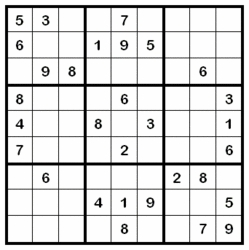
\includegraphics[scale=0.7]{sudo.jpg}
        \end{center}

    \end{enumerate}

    \begin{solution}
      Soient
      \[ x_{ijk} =
        \begin{cases}
          1 & \text{si la case }i, j\text{ a la valeur }k\\
          0 & \text{sinon}
        \end{cases}
      \]
      et $I = \{1,2,\ldots,9\}$
      \begin{enumerate}
        \item Le problème d'optimisation linéaire est le suivant
          \begin{align*}
            \min 1\\
            \sum_{j=1}^9 x_{ijk} & = 1 & \forall i,k \in I\\
            \sum_{i=1}^9 x_{ijk} & = 1 & \forall j,k \in I\\
            \sum_{i=r}^{r+2}\sum_{j=c}^{c+2} x_{ijk} & = 1
            & \forall r \in \{1,4,7\}, c \in \{1,4,7\}\\
            \sum_{k=1}^9 x_{ijk} & = 1 & \forall i,j \in I\\
            x & \leq 1\\
            x & \geq 0\\
            x & \text{ entiers}.
          \end{align*}
          La première (resp. deuxième) condition s'assure qu'on a bien complété
          les lignes (resp. les colonnes).
          La troisième fait de même pour les régions.
          La quatrième s'assure qu'on a complété un seul chiffre par
          case.
          Les 3 dernières s'assurent que $x$ contient des variables binaires.
        \item
          On va poser
          \begin{itemize}
            \item $a_i$ valant 1 si la ligne $i$ est complétée correctement
              et 0 sinon;
            \item $b_j$ valant 1 si la colonne $j$ est complétée correctement
              et 0 sinon;
            \item $c_{ij}$ valant 1 si la région donc un coin est en
              $(i,j)$ est complétée correctement
              et 0 sinon.
          \end{itemize}
          On peut alors exprimé le problème en le problème d'optimisation
          linéaire suivant
          \begin{align*}
            \max \sum_{i=1}^9 a_i + \sum_{j=1}^9 b_j +
            \sum_{r\in\{1,4,7\}}\sum_{c\in\{1,4,7\}} c_{rc}\\
            \sum_{j=1}^9 x_{ijk} & \leq 1 & \forall i,k \in I\\
            \sum_{i=1}^9 x_{ijk} & \leq 1 & \forall j,k \in I\\
            \sum_{i=r}^{r+2}\sum_{j=c}^{c+2} x_{ijk} & \leq 1
            & \forall r \in \{1,4,7\}, c \in \{1,4,7\}\\
            \sum_{k=1}^9 x_{ijk} & \leq 1 & \forall i,j \in I\\
            \sum_{k=1}^9\sum_{j=1}^9 x_{ijk}
            & \geq 9a_i & \forall i \in I\\
            \sum_{k=1}^9\sum_{i=1}^9 x_{ijk}
            & \geq 9b_j & \forall j \in I\\
            \sum_{k=1}^9\sum_{i=r}^{r+2}\sum_{j=c}^{c+2} x_{ijk}
            & \geq 9c_{rc}
            & \forall r \in \{1,4,7\}, c \in \{1,4,7\}\\
            (x,a,b,c) & \leq 1\\
            (x,a,b,c) & \geq 0\\
            (x,a,b,c) & \text{ entiers}.
          \end{align*}
      \end{enumerate}
    \end{solution}

  \item \textsc{OptiTv} lance un nouveau jeu sur nos écrans.  La
    dernière épreuve du jeu permet au gagnant de
    multiplier ses gains.

    Deux rails $A$ et $B$ traversent un plateau de jeu jonché
    d'obstacles.  Le but du joueur est de maximiser la masse
    totale
    de deux billes posées sur les rails qui pourront traverser le plateau.
    Pour ce faire, il peut décider de retirer
    certains obstacles du parcours, mais pour chaque obstacle
    enlevé, une pénalisation de $20$ grammes lui sera retranchée du résultat.
    Les règles du jeu sont les suivantes:
    \begin{enumerate}
      \item Le joueur a à sa disposition des billes de $10$,
        $20$, $30$, ..., $100$ grammes en quantité suffisante.  Il
        peut déposer $0$, $1$ ou $2$ billes sur le plateau
        (maximum une bille par rail), et chaque bille déposée doit
        traverser de part en part le plateau sous peine de
        disqualification.
      \item Pour assurer l'équilibre du plateau, la différence
        de masse entre les deux billes choisies ne peut pas excéder
        $20$ grammes. En particulier, si une seule bille traverse le
        plateau, sa masse ne peut pas être supérieure à $20$
        grammes.
      \item Si l'obstacle $1$ n'est pas ôté, une bille posée sur le rail $A$ ne
        peut pas traverser le plateau de jeu.
      \item Les obstacles $2$ et $3$ ne peuvent pas être retirés
        tous les deux ensemble.
      \item S'il souhaite retirer l'obstacle $2$ ou l'obstacle
        $4$, le joueur est obligé d'enlever d'abord les obstacles
        $1$ et $3$.
%        {\it \item Le joueur est obligé d'enlever au moins un des
%        obstacles parmi $2$ et $4$ ou d'enlever les deux obstacles
%        $1$ et $3$.}
      \item Les obstacles $3$ et $4$ déterminent conjointement
        la masse maximale de la bille qui pourra passer sur le rail $B$: le
        retrait de l'obstacle $3$ permet de faire passer $80$
        grammes et le retrait de l'obstacle $4$ autorise quant à lui $20$
        grammes.  En particulier, si ces deux obstacles sont
        retirés, une bille de $100$ grammes peut passer sur ce
        rail.
        %Quatre obstacles peuvent gêner la progression des billes.
    \end{enumerate}

    Formulez ce problème comme un problème d'optimisation linéaire
    en nombres entiers.  Vous ne devez pas résoudre ce
    problème.




    \begin{solution}
      \nosolution
    \end{solution}

  \item Vous disposez d'une somme de 96 Euros. Vous désirez acheter
    des boissons, disponibles en divers conditionnements.
    \begin{center}
      \begin{tabular}{|c|c|c|c|c|c|}
        \hline %\vspace{2pt}
        Boisson & A & B & C & D & E\\
        \hline
        Volume unitaire (litres) & 15 & 16 & 17 & 18 & 20\\
        \hline
        Prix unitaire (Euros) & 16 & 17 & 18 & 19 & 20\\
%\hline Nombre disponible & $\infty$ & $\infty$ & 6  & 4\\
        \hline
      \end{tabular}
    \end{center}
    Vous désirez acheter un volume le plus grand possible, sans
    dépasser votre budget.
    \begin{enumerate}
      \item Formulez ce problème comme un problème d'optimisation
        linéaire en nombres entiers.
      \item Combien de conditionnements de chaque type allez-vous acheter
        ? Détaillez votre raisonnement.
    \end{enumerate}

    \begin{solution}
      \nosolution
    \end{solution}

  \item Un transporteur est confronté au problème suivant : il ne
    peut transporter qu'une tonne de marchandises dans son véhicule,
    alors qu'une quantité supérieure à une tonne est disponible. Il
    reçoit les données suivantes de la part du comptable de
    l'entreprise, regroupant les quantités disponibles de chaque
    marchandise, ainsi que le bénéfice retiré par leurs ventes
    respectives.

    \begin{center}
      \begin{tabular}{|c|c|c|c|}
        \hline %\vspace{2pt}
        Marchandise & A & B & C\\
        \hline
        Quantité disponible (kg) & 900 & 240 & 560 \\
        \hline
        Bénéfice (euros/kg) & 15 & 17,5 & 14 \\
        \hline
      \end{tabular}
    \end{center}

    \begin{enumerate}
      \item D'après ces informations, formulez le problème d'optimisation
        linéaire correspondant et déterminez les quantités de A,B et C qui
        optimiseront le bénéfice réalisé par la vente du chargement et
        donnez la valeur de ce bénéfice.

        \vspace{6pt} Arrivé dans le hangar pour charger, le chauffeur
        réalise que les marchandises sont conditionnées en sacs, et qu'il
        est impensable de charger autres choses que des sacs complets.
        Voici les poids des sacs qui constituent le stock :
        \begin{center}
          \begin{tabular}{|c|c|c|c|}
            \hline %\vspace{2pt}
            Marchandise & A & B & C\\
            \hline
            Poids d'un sac (kg) & 60 & 80 & 20 \\
            \hline
          \end{tabular}
        \end{center}

      \item Reformulez le problème d'optimisation en tenant compte de ces
        dernières informations. Résolvez ce nouveau problème et comparez
        votre solution à la solution du cas~(a). Justifiez votre
        raisonnement.

      \item Le chauffeur (décidément malchanceux) se rend compte que le
        comptable a oublié de mentionner la marchandise D dont il reste
        trois sacs de 50 kg pouvant rapporter chacun 1000 Euros. A ce
        moment, il a déjà chargé neuf sacs de A et deux sacs de B, et ne
        compte pas les enlever de sa camionnette. Formulez le nouveau
        problème d'optimisation et expliquez une méthode de résolution
        "systématique" (par opposition à intuitive) de ce problème, sans la
        mener à terme.

    \end{enumerate}

    \begin{solution}
      \nosolution
    \end{solution}

\end{enumerate}


\end{document}
